%%%%%%%%%%%%%%%%%%%%%%%%%%%%%%%%%%%%%%%%%%%%%%%%%%%%%%%%%%%%%%%%%%%%%%%%
% Beamer Presentation - LaTeX - Template Version 1.0 (10/11/12)
% This template has been downloaded from: http://www.LaTeXTemplates.com
% License: % CC BY-NC-SA 3.0 (http://creativecommons.org/)
% Modified by Rahmat M. Samik-Ibrahim

% REV339 Sat 04 Sep 2021 12:50:36 WIB
% REV329 Tue 17 Aug 2021 18:37:09 WIB
% REV319 Mon 19 Jul 2021 23:57:40 WIB
% REV309 Mon 05 Jul 2021 15:32:10 WIB
% REV307 Wed 09 Jun 2021 15:52:17 WIB
% STARTX Wed Aug 24 19:34:33 WIB 2016
%%%%%%%%%%%%%%%%%%%%%%%%%%%%%%%%%%%%%%%%%%%%%%%%%%%%%%%%%%%%%%%%%%%%%%%%%

% PACKAGES AND THEMES ZCZC
\documentclass[xcolor=table, notheorems, hyperref={pdfpagelabels=false}]{beamer}
%%%%%%%%%%%%%%%%%%%%%%%%%%%%%%%%%%%%%%%%%%%%%%%%%%%%%%%%%%%%%%%%%%%%%%%%
% Beamer Presentation - LaTeX - Template Version 1.0 (10/11/12)
% This template has been downloaded from: http://www.LaTeXTemplates.com
% License: % CC BY-NC-SA 3.0 (http://creativecommons.org/)
% Modified by Rahmat M. Samik-Ibrahim
% REV316 Wed 14 Jul 2021 13:42:41 WIB
% REV217 Tue Feb  4 15:10:30 WIB 2020
% REV198 Wed Mar 13 16:39:02 WIB 2019
% REV006 Mon Jan 22 19:10:41 WIB 2018
% REV005 Mon Oct  2 14:45:07 WIB 2017
% START  Thu Aug 25 14:15:19 WIB 2016
%%%%%%%%%%%%%%%%%%%%%%%%%%%%%%%%%%%%%%%%%%%%%%%%%%%%%%%%%%%%%%%%%%%%%%%%%

%% ZCZC NNNN
\newtheorem{example}{Example}

%%%%%%%%%%%%%%%%%%%%%%%%%%%%%%%%%%%%%%%%%%%%%%%%%%%%%%%%%%%%%%%%%%%%%%%%%

\let\Tiny=\tiny
\mode<presentation> {
% The Beamer class comes with a number of default slide themes
% which change the colors and layouts of slides. Below this is a list
% of all the themes, uncomment each in turn to see what they look like.
%\usetheme{Boadilla}
\usetheme{Madrid}
% ZCZC %%%%%%%%%%%%%%%%%%%%%%%%%%%%%%%%%%%%%%%%%%%%%%%%%%%%%%%%%%%%%%%%%%
% \usetheme{default} \usetheme{AnnArbor} \usetheme{Antibes} \usetheme{Bergen}
% \usetheme{Berkeley} \usetheme{Berlin} \usetheme{CambridgeUS} 
% \usetheme{Copenhagen} \usetheme{Darmstadt} \usetheme{Dresden}
% \usetheme{Frankfurt} \usetheme{Goettingen} \usetheme{Hannover}
% \usetheme{Ilmenau} \usetheme{JuanLesPins} \usetheme{Luebeck}
% \usetheme{Malmoe} \usetheme{Marburg} \usetheme{Montpellier}
% \usetheme{PaloAlto} \usetheme{Pittsburgh} \usetheme{Rochester}
% \usetheme{Singapore} \usetheme{Szeged} \usetheme{Warsaw}
% NNNN %%%%%%%%%%%%%%%%%%%%%%%%%%%%%%%%%%%%%%%%%%%%%%%%%%%%%%%%%%%%%%%%%%
% As well as themes, the Beamer class has a number of color themes
% for any slide theme. Uncomment each of these in turn to see how it
% changes the colors of your current slide theme.
%\usecolortheme{orchid}
%\usecolortheme{rose}
%\usecolortheme{seagull}
%\usecolortheme{seahorse}
\usecolortheme{whale}
% ZCZC %%%%%%%%%%%%%%%%%%%%%%%%%%%%%%%%%%%%%%%%%%%%%%%%%%%%%%%%%%%%%%%%%%
%\usecolortheme{albatross} \usecolortheme{beaver} \usecolortheme{beetle}
%\usecolortheme{crane} \usecolortheme{dolphin} \usecolortheme{dove}
%\usecolortheme{fly} \usecolortheme{lily} \usecolortheme{wolverine}
% NNNN %%%%%%%%%%%%%%%%%%%%%%%%%%%%%%%%%%%%%%%%%%%%%%%%%%%%%%%%%%%%%%%%%%
% To remove the footer line in all slides uncomment this line
%\setbeamertemplate{footline} 
% To replace the footer line in all slides uncomment this line
%\setbeamertemplate{footline}[page number] 
% To remove the navigation symbols from the bottom uncomment this line
\setbeamertemplate{navigation symbols}{} 
}

\usepackage{array}       % ZCZC
\usepackage{amssymb}     % ZCZC
\usepackage{bold-extra}  % ZCZC
\usepackage{booktabs}    % Allows \toprule, \midrule and \bottomrule in tables
\usepackage{caption}
\usepackage[T1]{fontenc} % ZCZC << >>
\usepackage{graphicx}    % Allows including images
\usepackage{listings}    % listing
\usepackage{lmodern}     % ZCZC
\usepackage{perpage}     % reset footnote per page
\usepackage{geometry}    % ZCZC
\usepackage{adjustbox}   % ZCZC
\usepackage{multirow}    % ZCZC

% \definecolor{links}{HTML}{2A1B81}
\definecolor{links}{HTML}{0011FF}
\hypersetup{colorlinks,linkcolor=,urlcolor=links}

% \usepackage{xcolor}
% \usepackage[colorlinks = true,
%             linkcolor = blue,
%             urlcolor  = blue,
%             citecolor = blue,
%             anchorcolor = blue]{hyperref}

\captionsetup[table]{name=Tabel}
\makeatletter
\def\input@path{{src/}}
\makeatother
\graphicspath{{src/}}      % src directory
\MakePerPage{footnote}     % reset page

% NNNN %%%%%%%%%%%%%%%%%%%%%%%%%%%%%%%%%%%%%%%%%%%%%%%%%%%%%%%%%%%%%%%%%%

%% % XXXXXXXXXXXXXXXXXXXXXXXXXXXXXXXXXXXXXXXXXXXXXXXXXXXXXXXXXXXXXXXXXXXXXXXXXX
%% % The short title appears at the bottom of every slide, 
%% % the full title is only on the title page
%% \title[Judul Pendek]{Judul Panjang dan Lengkap} 
%% \author{Cecak bin Kadal}
%% \institute[UILA]
%% {
%% University of Indonesia at Lenteng Agung \\ 
%% \medskip
%% \textit{cecak@binKadal.com}
%% }
%% \date{REV00 24-Aug-2016}
%% % \date{\today}
%% 

%% % XXXXXXXXXXXXXXXXXXXXXXXXXXXXXXXXXXXXXXXXXXXXXXXXXXXXXXXXXXXXXXXXXXXXXXXXXX
%% \begin{document}
%% \section{Judul}
%% \begin{frame}
%% \titlepage
%% \end{frame}
%% 
%% % XXXXXXXXXXXXXXXXXXXXXXXXXXXXXXXXXXXXXXXXXXXXXXXXXXXXXXXXXXXXXXXXXXXXXXXXXX
%% \section{Agenda}
%% \begin{frame}
%% \frametitle{Agenda}
%% % Throughout your presentation, if you choose to use \section{} and 
%% % \subsection{} commands, these will automatically be printed on 
%% % this slide as an overview of your presentation
%% \tableofcontents 
%% \end{frame}
%% 
%% % XXXXXXXXXXXXXXXXXXXXXXXXXXXXXXXXXXXXXXXXXXXXXXXXXXXXXXXXXXXXXXXXXXXXXXXXXX
%% \section{UUD dan Pancasila}
%% \subsection{UUD}
%% \begin{frame}
%% \frametitle{Pembukaan}
%% Bahwa sesungguhnya kemerdekaan itu ialah hak segala bangsa dan oleh 
%% sebab itu, maka penjajahan diatas dunia harus dihapuskan karena 
%% tidak sesuai dengan perikemanusiaan dan perikeadilan.
%% \\~\\
%% Atas berkat rahmat Allah Yang Maha Kuasa dan dengan didorongkan oleh 
%% keinginan luhur, supaya berkehidupan kebangsaan yang bebas, maka 
%% rakyat Indonesia menyatakan dengan ini kemerdekaannya.
%% \end{frame}
%% 
%% % XXXXXXXXXXXXXXXXXXXXXXXXXXXXXXXXXXXXXXXXXXXXXXXXXXXXXXXXXXXXXXXXXXXXXXXXXX
%% \begin{frame}
%% \frametitle{Alenia Ketiga}
%% Kemudian daripada itu untuk membentuk suatu pemerintah negara Indonesia 
%% yang melindungi segenap bangsa Indonesia dan seluruh tumpah darah Indonesia 
%% dan untuk memajukan kesejahteraan umum, mencerdaskan kehidupan bangsa, dan 
%% ikut melaksanakan ketertiban dunia yang berdasarkan kemerdekaan, perdamaian 
%% abadi dan keadilan sosial, maka disusunlah kemerdekaan kebangsaan Indonesia 
%% itu dalam suatu Undang-Undang Dasar negara Indonesia, yang terbentuk dalam 
%% suatu susunan negara Republik Indonesia yang berkedaulatan rakyat dengan 
%% berdasar kepada:
%% \begin{itemize}
%% \item Ketuhanan Yang Maha Esa,
%% \item kemanusiaan yang adil dan beradab,
%% \item persatuan Indonesia,
%% \item dan kerakyatan yang dipimpin oleh hikmat kebijaksanaan 
%%       dalam permusyawaratan/ perwakilan,
%% \item serta dengan mewujudkan suatu keadilan sosial bagi seluruh rakyat 
%%       Indonesia.
%% \end{itemize}
%% \end{frame}
%% 
%% % XXXXXXXXXXXXXXXXXXXXXXXXXXXXXXXXXXXXXXXXXXXXXXXXXXXXXXXXXXXXXXXXXXXXXXXXXX
%% \subsection{Pancasila}
%% \begin{frame}
%% \frametitle{Tujuh Kunci Pokok}
%% \begin{block}{Pertama - Kedua - Ketiga}
%% Indonesia ialah negara berdasarkan hukum.
%% Sistem konstitusional.
%% Kekuasaan negara tertinggi di tangan MPR.
%% \end{block}
%% 
%% \begin{block}{Keempat - Kelima}
%% Presiden adalah penyelenggara pemerintahan tertinggi di bawah MPR.
%% Adanya pengawasan DPR.
%% \end{block}
%% 
%% \begin{block}{Keenam}
%% Menteri negara adalah pembantu presiden dan tidak bertanggung jawab 
%% kepada DPR.
%% \end{block}
%% 
%% \begin{block}{Ketujuh}
%% Kekuasaan kepala negara tidak tak tebatas.
%% \end{block}
%% 
%% \end{frame}
%% 
%% % XXXXXXXXXXXXXXXXXXXXXXXXXXXXXXXXXXXXXXXXXXXXXXXXXXXXXXXXXXXXXXXXXXXXXXXXXX
%% \section{Rupa-rupa}
%% \subsection{Kolom}
%% \begin{frame}
%% \frametitle{Kolom}
%% % The "c" option specifies centered vertical alignment 
%% % while the "t" option is used for top vertical alignment
%% \begin{columns}[c] 
%% % Left column and width
%% \column{.45\textwidth} 
%% \textbf{Heading}
%% \begin{enumerate}
%% \item Satu-satu
%% \item Dua-dua
%% \item Tiga-tiga
%% \item Satu-dua-tiga
%% \end{enumerate}
%% 
%% % Right column and width
%% \column{.5\textwidth}
%% Satu-satu~\dots{} aku sayang ibu!
%% Dua-dua~\ldots{} juga sayang ayah!
%% Tiga-tiga~\ldots{} sayang adik kakak!
%% Satu-dua-tiga~\ldots{} sayang semuanya!
%% 
%% \end{columns}
%% \end{frame}
%% 
%% % XXXXXXXXXXXXXXXXXXXXXXXXXXXXXXXXXXXXXXXXXXXXXXXXXXXXXXXXXXXXXXXXXXXXXXXXXX
%% \subsection{Tabel}
%% \begin{frame}
%% \frametitle{Tabel}
%% \begin{table}
%% \begin{tabular}{l l l}
%% \toprule
%% \textbf{Nama} & \textbf{NPM} & \textbf{Tanggal Lahir}\\
%% \midrule
%% Cecak bin Kadal & 1234567890 & 1 Jan 2015 \\
%% Aneh bin Ajaib  & 0987654321 & 31 Des 2014 \\
%% \bottomrule
%% \end{tabular}
%% \caption{Keterangan Tabel}
%% \end{table}
%% \end{frame}
%% 
%% % XXXXXXXXXXXXXXXXXXXXXXXXXXXXXXXXXXXXXXXXXXXXXXXXXXXXXXXXXXXXXXXXXXXXXXXXXX
%% \subsection{Teori}
%% \begin{frame}
%% \frametitle{Teori}
%% \begin{theorem}[Teori Satu Batu]
%% $E = mc^2$
%% \end{theorem}
%% \end{frame}
%% 
%% % XXXXXXXXXXXXXXXXXXXXXXXXXXXXXXXXXXXXXXXXXXXXXXXXXXXXXXXXXXXXXXXXXXXXXXXXXX
%% \subsection{Verbatim}
%% % Need to use the fragile option when verbatim is used in the slide
%% \begin{frame}[fragile] 
%% \frametitle{Verbatim}
%% \begin{example}[Teori Satu Batu]
%% \begin{verbatim}
%% \begin{theorem}[Teori Satu Batu]
%% $E = mc^2$
%% \end{theorem}
%% \end{verbatim}
%% \end{example}
%% \end{frame}
%% 
%% % XXXXXXXXXXXXXXXXXXXXXXXXXXXXXXXXXXXXXXXXXXXXXXXXXXXXXXXXXXXXXXXXXXXXXXXXXX
%% \subsection{Gambar}
%% \begin{frame}
%% \frametitle{Gambar}
%% \begin{figure}
%% \includegraphics[width=0.5\linewidth]{2}
%% \caption{Ini Gambar JPG}
%% \end{figure}
%% \end{frame}
%% 
%% % XXXXXXXXXXXXXXXXXXXXXXXXXXXXXXXXXXXXXXXXXXXXXXXXXXXXXXXXXXXXXXXXXXXXXXXXXX
%% \subsection{Rujukan}
%% % Need to use the fragile option when verbatim is used in the slide
%% \begin{frame}[fragile] 
%% \frametitle{Rujukan dan Kutipan}
%% Contoh penggunaan \verb|\cite| ketika mengutip\cite{p1}.
%% Perhatian: Beamer tidak mengerti \verb|\BibTeX|~\ldots
%% \footnotesize{
%%   \begin{thebibliography}{99} 
%%   \bibitem[Smith, 2012]{p1} John Smith (2012)
%%      \newblock Katak dalam Tempurung
%%      \newblock \emph{Jurnal Kelapa dan Amfibi} 12(3), 45 -- 678.
%%   \end{thebibliography}
%% }
%% \end{frame}
%% 
%% % XXXXXXXXXXXXXXXXXXXXXXXXXXXXXXXXXXXXXXXXXXXXXXXXXXXXXXXXXXXXXXXXXXXXXXXXXX
%% \subsection{Selesai}
%% \begin{frame}
%% \Huge{\centerline{Selesai}}
%% \end{frame}
%% 
%% % XXXXXXXXXXXXXXXXXXXXXXXXXXXXXXXXXXXXXXXXXXXXXXXXXXXXXXXXXXXXXXXXXXXXXXXXXX
%% \end{document}

\newcommand{\revision}{REV362 21-Nov-2021}
% w! tmptmp
% REV362 Sun 21 Nov 2021 17:54:07 WIB
% REV359 Sat 30 Oct 2021 14:42:29 WIB
% REV349 Sun 26 Sep 2021 09:13:27 WIB
% REV339 Sat 04 Sep 2021 12:50:36 WIB
% REV329 Tue 17 Aug 2021 20:15:00 WIB
% STARTS Wed 24 Aug 2016 19:34:33 WIB
%%%%%%%%%%%%%%%%%%%%%%%%%%%%%%%%%%%%%
\newcommand{\kopikopi}{\textcopyright{}2016-2021 VauLSMorg}



% XXXXXXXXXXXXXXXXXXXXXXXXXXXXXXXXXXXXXXXXXXXXXXXXXXXXXXXXXXXXXXXXXXXXXXXXXX
% The short title appears at the bottom of every slide, 
% the full title is only on the title page
% \date{\today}
\title[\kopikopi]
{CSF2600505 Sistem Operasi   \\
CSGE602055 Operating Systems \\ 
Week 00:
Overview 1} 
\author{Rahmat M. Samik-Ibrahim (ed.)}
\institute[UI]
{
University of Indonesia\\ 
\medskip
\url{https://os.vlsm.org/Slides/os00.pdf}
\\ \texttt{Always check for the latest revision!}
}
\date{\revision}

% XXXXXXXXXXXXXXXXXXXXXXXXXXXXXXXXXXXXXXXXXXXXXXXXXXXXXXXXXXXXXXXXXXXXXXXXXX
\begin{document}

\lstset{
basicstyle=\ttfamily\tiny, % \tiny \small \footnotesize 
breakatwhitespace=true,
language=C,
columns=fullflexible,
keepspaces=true,
breaklines=true,
tabsize=3, 
showstringspaces=false,
extendedchars=true}

\section{Start}
\begin{frame}
\titlepage
\end{frame}

% XXXXXXXXXXXXXXXXXXXXXXXXXXXXXXXXXXXXXXXXXXXXXXXXXXXXXXXXXXXXXXXXXXXXXXXXXX

\label{laman}
%%%%%%%%%%%%%%%%%%%%%%%%%%%%%%%%%%%%%%%%%%%%%%%%%%%%%%%%%%%%%%%%%%%%%%%%%
% REV352 Sun 10 Oct 2021 09:56:47 WIB
% REV341 Sun 05 Sep 2021 23:30:00 WIB
% REV333 Thu 26 Aug 2021 08:52:24 WIB
% REV328 Sat 14 Aug 2021 06:32:08 WIB
% REV272 Mon 01 Mar 2021 12:02:09 WIB
% START0 Sat Sep  2 10:51:33 WIB 2017
%%%%%%%%%%%%%%%%%%%%%%%%%%%%%%%%%%%%%%%%%%%%%%%%%%%%%%%%%%%%%%%%%%%%%%%%%

\begin{frame}[fragile]
\section{Schedule}
\frametitle{OS212\footnote{%
) This information will be on \textbf{EVERY} page two (2) of this course material.}): 
Operating Systems 2021 - 2}
\scalebox{0.73}{%
\begin{tabular}{|c|c|c|c|}
\hline
\makebox[106pt]{OS A} & \makebox[106pt]{OS B} & \makebox[107pt]{OS C} & \makebox[107pt]{OS INT} \\
\hline
\multicolumn{4}{|c|}{Every first day of the Week, \textbf{Quiz\#1:} (07:40-07:50) and \textbf{Quiz\#2:} 07:20-07:40} \\
\hline
Monday/Thursday & Monday/Thursday & Monday/Thursday & Monday/Wednesday   \\
13:00 --- 14:40  & 15:00 --- 16:40\footnote{) \textbf{OS B:} Week00-Week05 (RMS); Week06-Week10 (MAM).} &
                                      13:00 --- 14:40 & 08:00 --- 09:40  \\
14:00 --- finish & 16:00 --- finish & 13:00 --- 14:40 & 09:00 --- finish \\
\hline
\end{tabular}
}

\vspace{5pt}

\scalebox{0.73}{%
\begin{tabular}{|c|c|l|l|}
\hline
\textbf{Week} & \textbf{Schedule \& Deadline}\footnote{%
    ) The \textbf{DEADLINE} of Week 00 is 05 Sep 2021,
      whereas the \textbf{DEADLINE} of Week 01 is 12 Sep 2021, and so on...%
    })& \textbf{Topic} & \textbf{OSC10}\footnote{%
    ) Silberschatz et. al.: \textbf{Operating System Concepts}, $10^{th}$ Edition, 2018.}) \\
\hline
Week 00  & 30 Aug - 05 Sep 2021 & Overview 1, Virtualization \& Scripting & Ch. 1, 2, 18. \\
Week 01  & 06 Sep - 12 Sep 2021 & Overview 2, Virtualization \& Scripting & Ch. 1, 2, 18. \\
Week 02  & 13 Sep - 19 Sep 2021 & Security, Protection, Privacy, \& C-language.  & Ch. 16, 17. \\
Week 03  & 20 Sep - 26 Sep 2021 & File System \& FUSE  & Ch. 13, 14, 15. \\
Week 04  & 27 Sep - 03 Oct 2021 & Addressing, Shared Lib, \& Pointer & Ch. 9. \\
Week 05  & 04 Oct - 10 Oct 2021 & Virtual Memory & Ch. 10. \\
\hline
Week 06  & 11 Oct - 31 Oct 2021 & Concurrency: Processes \& Threads & Ch. 3, 4. \\
Week 07  & 01 Nov - 07 Nov 2021 & Synchronization \& Deadlock & Ch. 6, 7, 8. \\
Week 08  & 08 Nov - 14 Nov 2021 & Scheduling + W06/W07 & Ch. 5. \\
Week 09  & 15 Nov - 21 Nov 2021 & Storage, Firmware, Bootloader, \& Systemd & Ch. 11. \\
Week 10  & 22 Nov - 28 Nov 2021 & I/O \& Programming & Ch. 12. \\%
% MidTerm  & 00 XXX 2020 (XX:XX-XX:XX) & MidTerm (UTS) & \cellcolor{red!44} TBA! \\
% Reserved & 00 XXX - 00 XXX 2020 & Q \& A & \\
% Final    & 00 XXX 2020 XX:XX & First Part Final  (UAS tahap I)  & \cellcolor{red!44} This schedule is   \\
% Extra    & NA & No Extra assignment & \cellcolor{red!44} subject to change. \\
\hline
\end{tabular}
}
\end{frame}

\begin{frame}[fragile]
\frametitle{\textbf{STARTING POINT} --- 
{
\definecolor{links}{HTML}{FDEE00}
\hypersetup{colorlinks,linkcolor=,urlcolor=links}
\url{https://os.vlsm.org/}
}
}
\begin{itemize}
\item[$\square$] \textbf{Text Book} ---
                 Any recent/decent OS book. Eg. (\textbf{OSC10}) Silberschatz et. al.: 
                 \textbf{Operating System Concepts}, $10^{th}$ Edition, 2018.
                 See also \url{https://www.os-book.com/OS10/}.
\item[$\square$] \textbf{Resources}
\begin{itemize}
\item[$\square$] \href{https://scele.cs.ui.ac.id/course/view.php?id=3268}{\textbf{SCELE OS212}} ---
\url{https://scele.cs.ui.ac.id/course/view.php?id=3268}.\\
The enrollment key is \textbf{XXX}.
\item[$\square$] \textbf{Download Slides and Demos from GitHub.com} \\
\url{https://github.com/UI-FASILKOM-OS/SistemOperasi/}:

                 {\scriptsize%
                 \href{https://os.vlsm.org/Slides/os00.pdf}{\texttt{os00.pdf} (W00)},
                 \href{https://os.vlsm.org/Slides/os01.pdf}{\texttt{os01.pdf} (W01)},
                 \href{https://os.vlsm.org/Slides/os02.pdf}{\texttt{os02.pdf} (W02)},
                 \href{https://os.vlsm.org/Slides/os03.pdf}{\texttt{os03.pdf} (W03)},

                 \href{https://os.vlsm.org/Slides/os04.pdf}{\texttt{os04.pdf} (W04)},
                 \href{https://os.vlsm.org/Slides/os05.pdf}{\texttt{os05.pdf} (W05)},
                 \href{https://os.vlsm.org/Slides/os06.pdf}{\texttt{os06.pdf} (W06)},
                 \href{https://os.vlsm.org/Slides/os07.pdf}{\texttt{os07.pdf} (W07)},

                 \href{https://os.vlsm.org/Slides/os08.pdf}{\texttt{os08.pdf} (W08)},
                 \href{https://os.vlsm.org/Slides/os09.pdf}{\texttt{os09.pdf} (W09)},
                 \href{https://os.vlsm.org/Slides/os10.pdf}{\texttt{os10.pdf} (W10)}.
                 }
\item[$\square$] \textbf{Problems}\\
                 {\scriptsize% 
                 \href{https://rms46.vlsm.org/2/195.pdf}{\texttt{195.pdf} (W00)},
                 \href{https://rms46.vlsm.org/2/196.pdf}{\texttt{196.pdf} (W01)},
                 \href{https://rms46.vlsm.org/2/197.pdf}{\texttt{197.pdf} (W02)},
                 \href{https://rms46.vlsm.org/2/198.pdf}{\texttt{198.pdf} (W03)},\\
                 \href{https://rms46.vlsm.org/2/199.pdf}{\texttt{199.pdf} (W04)},
                 \href{https://rms46.vlsm.org/2/200.pdf}{\texttt{200.pdf} (W05)},
                 \href{https://rms46.vlsm.org/2/201.pdf}{\texttt{201.pdf} (W06)},
                 \href{https://rms46.vlsm.org/2/202.pdf}{\texttt{202.pdf} (W07)},\\
                 \href{https://rms46.vlsm.org/2/203.pdf}{\texttt{203.pdf} (W08)},
                 \href{https://rms46.vlsm.org/2/204.pdf}{\texttt{204.pdf} (W09)},
                 \href{https://rms46.vlsm.org/2/205.pdf}{\texttt{205.pdf} (W10)}.}
\item[$\square$] \textbf{LFS} --- \url{http://www.linuxfromscratch.org/lfs/view/stable/}
\item[$\square$] \textbf{OSP4DISS} --- \url{https://osp4diss.vlsm.org/}
\item[$\square$] \textbf{DOIT} --- \url{https://doit.vlsm.org/001.html}
\end{itemize}
\end{itemize}
\end{frame}



% XXXXXXXXXXXXXXXXXXXXXXXXXXXXXXXXXXXXXXXXXXXXXXXXXXXXXXXXXXXXXXXXXXXXXXXXXX
% Throughout your presentation, if you choose to use \section{} and 
% \subsection{} commands, these will automatically be printed on 
% this slide as an overview of your presentation
\section{Agenda}
\begin{frame}{Outline}
  \frametitle{Agenda}
  \tableofcontents[sections={1-16}]
\end{frame}
\begin{frame}
   \frametitle{Agenda (2)}
   \tableofcontents[sections={17-}]
\end{frame}

% XXXXXXXXXXXXXXXXXXXXXXXXXXXXXXXXXXXXXXXXXXXXXXXXXXXXXXXXXXXXXXXXXXXXXXXXXX
\section{How to contact the Lecturer}
\begin{frame}[fragile]
\frametitle{How to contact the Lecturer}
\begin{itemize}
\item \textbf{Always introduce yourself}. State your ''\texttt{GitHubAccount}'', ''\texttt{Name}'',
      ''\texttt{Student ID}'', and ''\texttt{OS class}''.
\item Post a question/query on 
\href{https://scele.cs.ui.ac.id/course/view.php?id=3268}{\textbf{SCELE OS212}} ---
(The enrollment key is \textbf{XXX}):
\href{https://scele.cs.ui.ac.id/course/view.php?id=3268}{https://scele.cs.ui.ac.id/course/view.php?id=3268}.
\item For SIAK related questions, use email:\\
(Subject:\textbf{[HELP]}) \texttt{operatingsystems(AT)vlsm.org}. 
\item \textbf{DO NOT} send an email for assignment-related questions.
\end{itemize}

\begin{figure}

\includegraphics[width=0.32\linewidth]{os00-pib}
\caption{Never ever whine and pretend like 
         this\footnote{''Puss in Boot'' is a DreamWorks/Paramount Picture character.}!}
\end{figure}
\end{frame}

% XXXXXXXXXXXXXXXXXXXXXXXXXXXXXXXXXXXXXXXXXXXXXXXXXXXXXXXXXXXXXXXXXXXXXXXXXX
\section{Assessment}
\begin{frame}
\frametitle{Assessment}
\begin{itemize}
\item \textbf{4 SKS} (Units) means 12 hours per week!
\begin{itemize}
\item You need to log your weekly activities!
\end{itemize}
\item \textbf{11} (weekly) assignments @ 11.11 points.
\begin{itemize}
\item Assignments will vary from week to week.
\item The assignment deadline will be by the end of every week. See page \pageref{laman}.
\item See the checklist at the end of this presentation.
\end{itemize}
\item Final grade: the sum of the best 9 out of 11 assignments.
\begin{tabular}{l l l l}
\hline
85 - ... = A & 80 - 85 = A- & 75 - 80 = B+ & 70 - 75 = B \\
65 - 70 = B-      & 60 - 65 = C+ & 55 - 60 = C  & 
50 - 55 = D or C\footnote{Terms and conditions apply --- void where prohibited by law.}  \\
40 - 50 = D  & 30 - 40 = E  & 20 - 30 = \small E & 00 - 20 = \tiny E   \\
\hline
\end{tabular}

\begin{itemize}
\item \textbf{C-2C:} up to 5 points.
\begin{itemize}
\item Only if your grade is between 50.00 and 55.00, and you have a ''good'' track record.
\end{itemize}
\item Check your points regularly at \url{https://academic.ui.ac.id/} and 
      \textbf{DO NOT COMPLAIN} weeks after! See also, \url{https://os.vlsm.org/Log/}.
\end{itemize}
\end{itemize}

\end{frame}

% XXXXXXXXXXXXXXXXXXXXXXXXXXXXXXXXXXXXXXXXXXXXXXXXXXXXXXXXXXXXXXXXXXXXXXXXXX
\section{The Three-Strikes Rule}
\begin{frame}[fragile]
\frametitle{The Three-Strikes Rule}

\begin{figure}
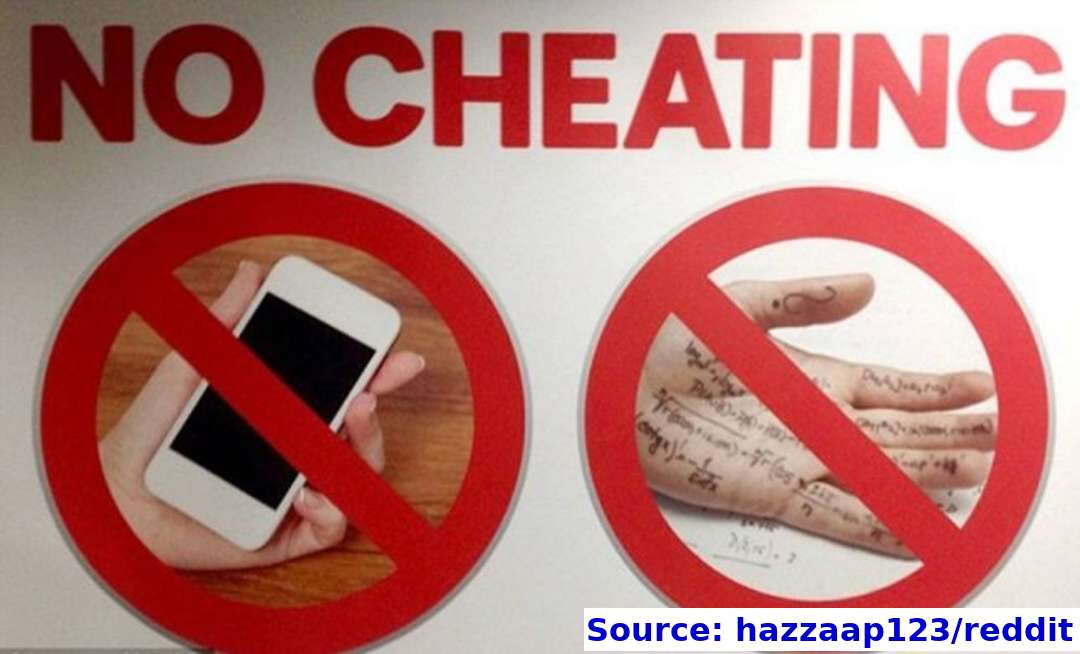
\includegraphics[width=0.37\linewidth]{os-cheating}
\end{figure}

\begin{itemize}
\item All major academic rules violations will be handled directly by the Faculty of Computer Science,
University of Indonesia.
\item ''Accidents'' may happen. There will be warnings for the first two minor violations.
\item Your final grade will be reduced for the third warning.
\item Your final grade will be reduced to "D" for the fourth warning.
\item Five (5) or more warnings will be considered as a significant academic-rules violation.
\end{itemize}

\end{frame}

% XXXXXXXXXXXXXXXXXXXXXXXXXXXXXXXXXXXXXXXXXXXXXXXXXXXXXXXXXXXXXXXXXXXXXXXXXX
\begin{frame}[fragile]
\frametitle{AIN'T DIFFICULT, lah!}
\begin{figure}
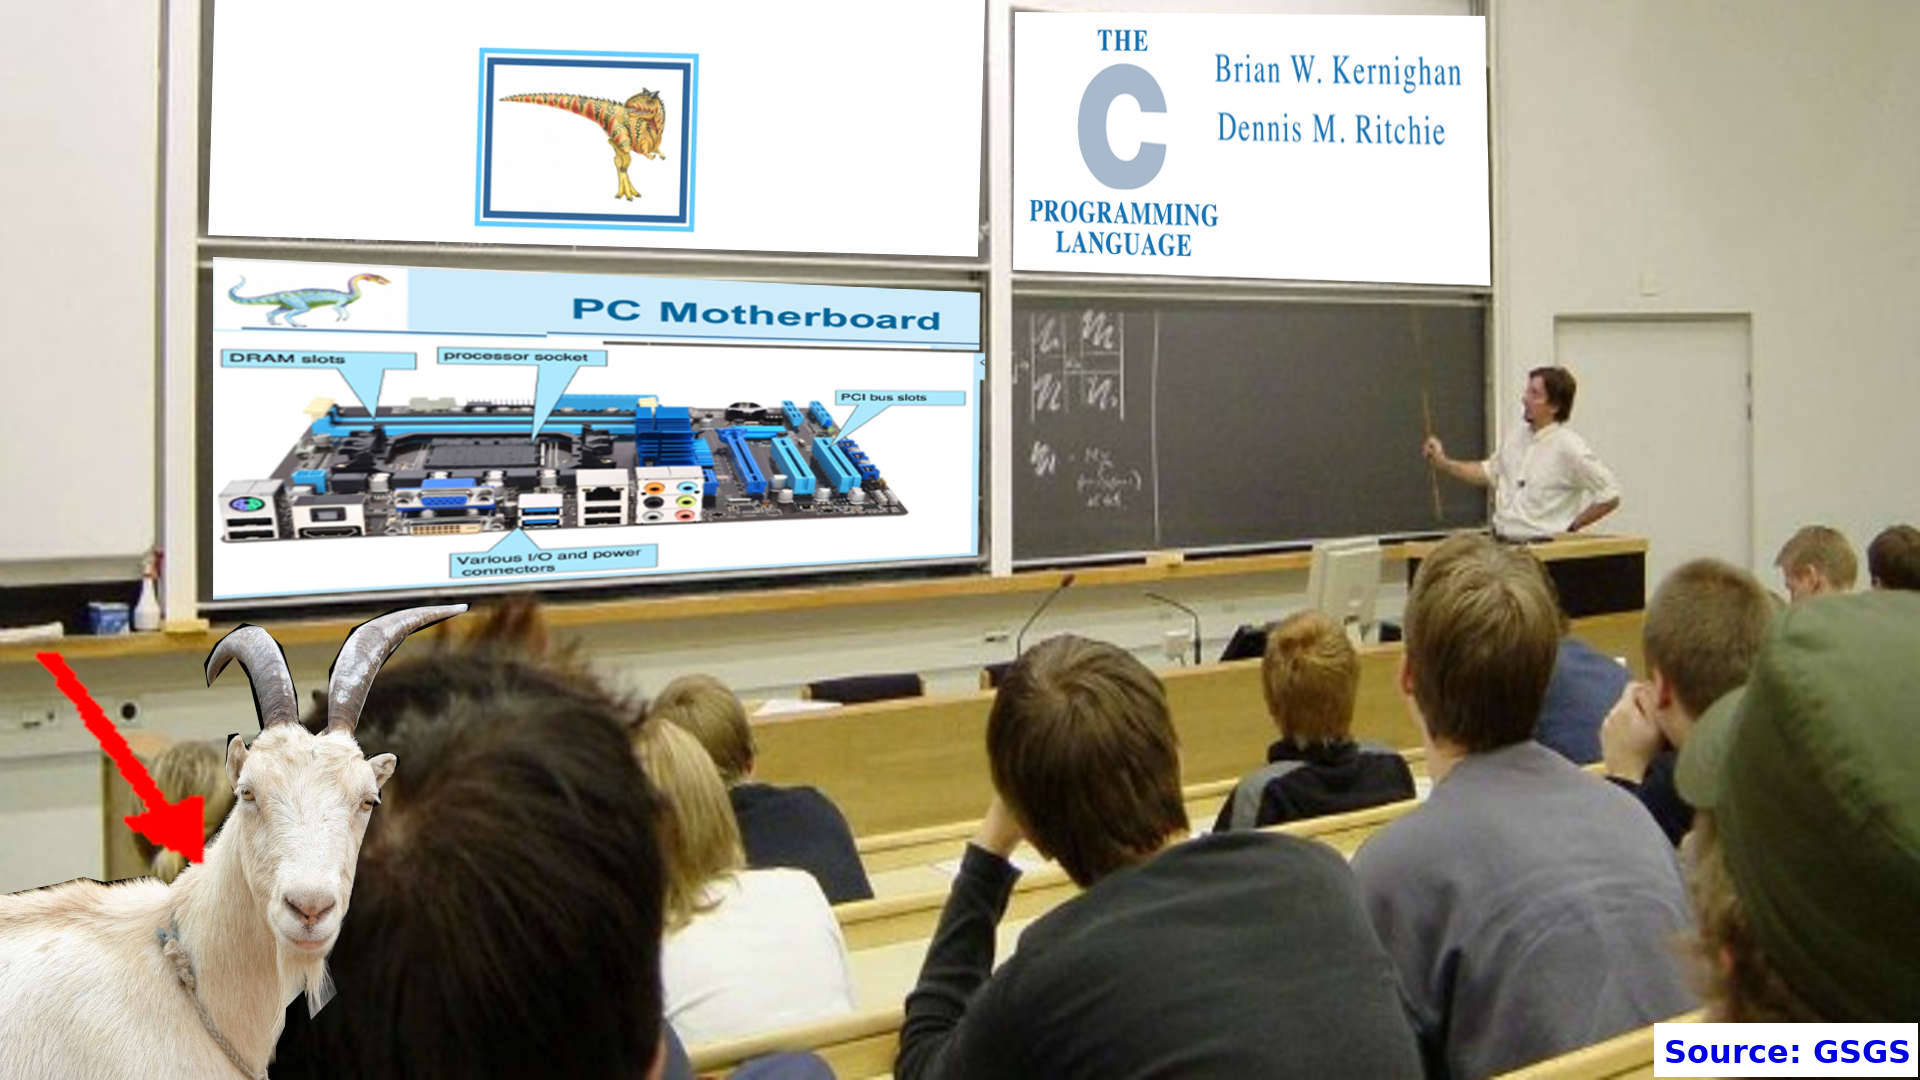
\includegraphics[width=0.90\linewidth]{os-kambing-kuliah-c}
\caption{Even this Goat will get ''C'' at the end of the semester!}
\end{figure}
\end{frame}

% XXXXXXXXXXXXXXXXXXXXXXXXXXXXXXXXXXXXXXXXXXXXXXXXXXXXXXXXXXXXXXXXXXXXXXXXXX
\begin{frame}[fragile]
\frametitle{Prelude: Daisy Bell -- Bicycle Built for Two}
\begin{tabular}{cc}
\begin{minipage}{45mm}
\vspace{1pt}
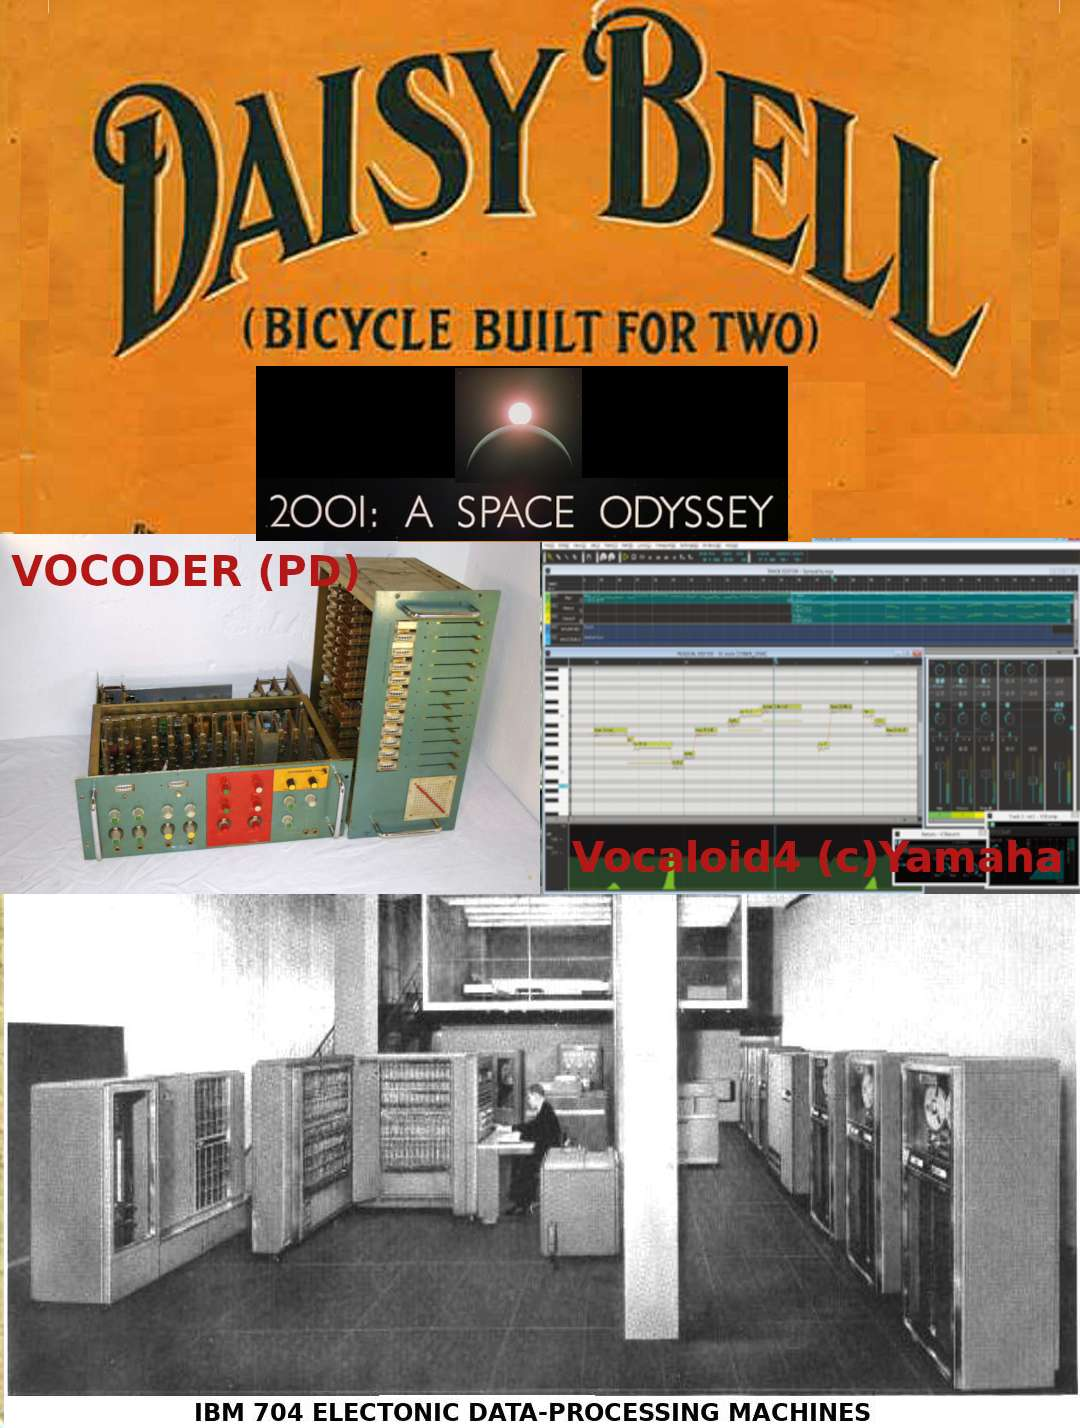
\includegraphics[width=0.99\linewidth]{os-daisybell}
\end{minipage}
&
\begin{minipage}{65mm}
\vspace{1pt}
\begin{verbatim}
Daisy, Daisy,
Give me your answer, do!
I'm half crazy,
All for the love of you!
It won't be a stylish marriage,
I can't afford a carriage,
But you'll look sweet on the seat
Of a bicycle built for two!
\end{verbatim}
\end{minipage}
\\
\end{tabular}
\\[5mm]

A choir (emulation) of VOCODER (pre WW2), IBM704 (1950s) and  Vocaloid4 (2014).
See also the classical movie "\textbf{2001: A Space Odyssey}" and YouTube: \url{https://youtu.be/TXK_cE9AqAI}.
\end{frame}

% XXXXXXXXXXXXXXXXXXXXXXXXXXXXXXXXXXXXXXXXXXXXXXXXXXXXXXXXXXXXXXXXXXXXXXXXXX
\begin{frame}
\frametitle{IBM 704 at Los Alamos National Laboratory in the 1950s}
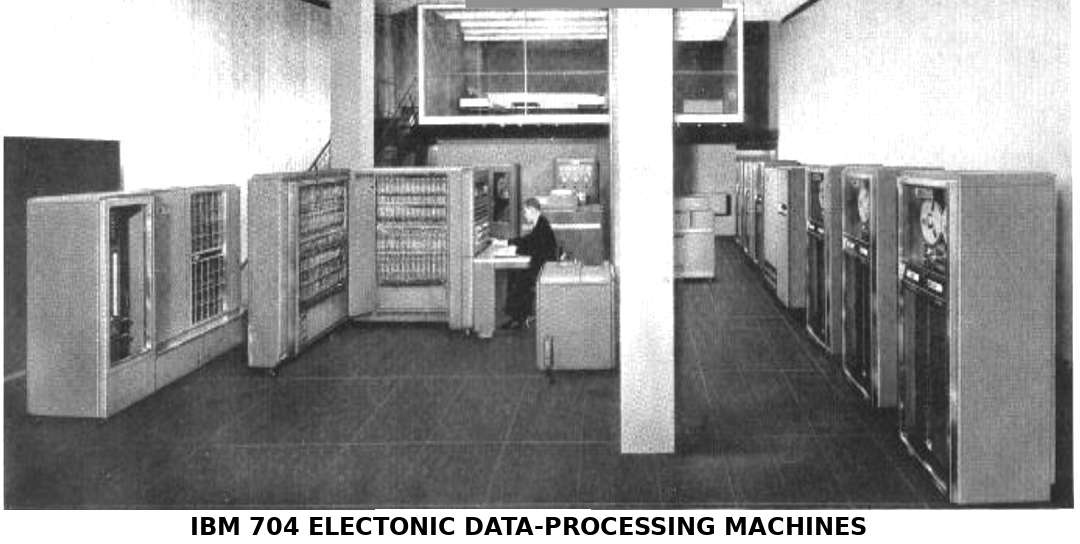
\includegraphics[width=0.90\linewidth]{os-ibm704}

Estimate price (2020 value): USD 8,000,000.

Weight: 8800 kg --- Electricity: ca. 200 kWatt --- 42000 flops --- 
128 kbytes (eq.) core memory --- 64 kbytes (eq.) drum memory --- 3 Mbytes (eq.) Tape Unit.

\end{frame}

% XXXXXXXXXXXXXXXXXXXXXXXXXXXXXXXXXXXXXXXXXXXXXXXXXXXXXXXXXXXXXXXXXXXXXXXXXX
\begin{frame}
\frametitle{QS855, 256GB, 12 GB, 48+12 MP, 6.4'', 4000 mAh}
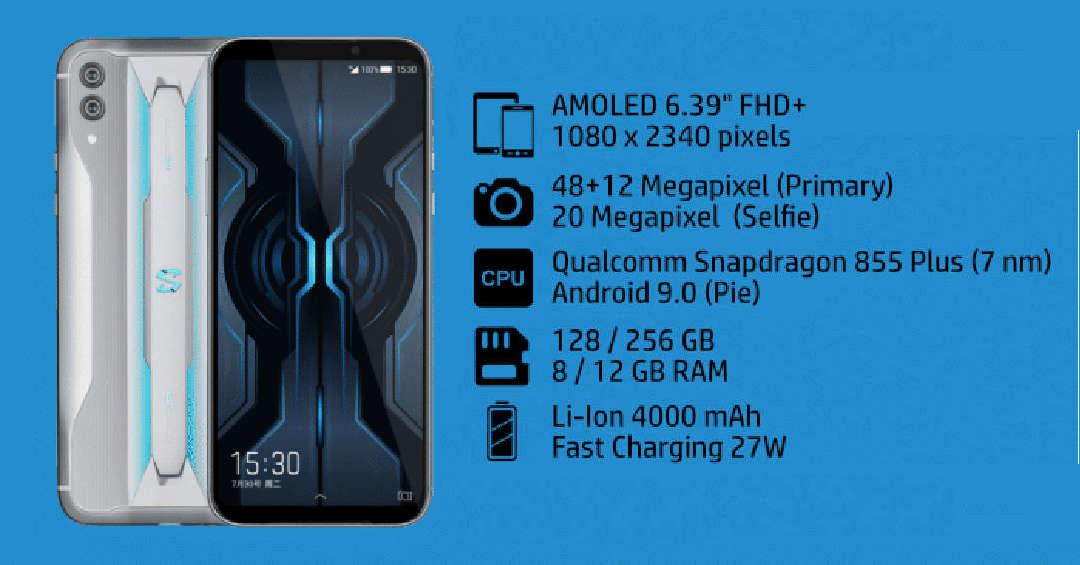
\includegraphics[width=0.90\linewidth]{os-xiaomi-black-shark-2-pro}

Estimate price (2020 value): Rp. 8,000,000.

\end{frame}

% XXXXXXXXXXXXXXXXXXXXXXXXXXXXXXXXXXXXXXXXXXXXXXXXXXXXXXXXXXXXXXXXXXXXXXXXXX
\section{LFS: Linux From Scratch}
\begin{frame}
\frametitle{LFS: Linux From Scratch (Week 00 --- Week 10)}
\begin{itemize}
\item \href{https://youtu.be/jEoM3qan9Gs}{THIS IS HOW WE DOIT!}
\item \url{http://www.linuxfromscratch.org/lfs/view/stable/}
\item To build a GNU/Linux system from scratch (source code).
\item To learn a GNU/Linux system inside out.
\item To use a Virtual Machine.
\item A Chicken and Egg dependency problem:
\begin{itemize}
\item It would be best if you had the tools to build an Operating System.
\item You need an Operating System to build tools.
\item To build a cross-toolchain (compiler and its libraries).
\item To build cross utilities using the cross-toolchain.
\item To build an Operating System in a chroot environment.
\item To do iterations (if necessary).
\end{itemize}
\item How deep would you like to know of a ''real'' Operating System?
\item Whatever, however, from Week 00 to Week 10!
\item \textbf{YOU} decide!
\end{itemize}
\end{frame}

% XXXXXXXXXXXXXXXXXXXXXXXXXXXXXXXXXXXXXXXXXXXXXXXXXXXXXXXXXXXXXXXXXXXXXXXXXX
\section{Week 00: Review}
\begin{frame}
\frametitle{Week 00: Review}

\begin{itemize}
\item{What is an Operating System?}
\item Why taking an Operating System class?
\end{itemize}

\begin{table}
\scalebox{0.8}{%
\begin{tabular}{| c |}
\hline \\ [1mm]
Business Goal \\
\vline \\ [2mm]
Application \\
\vline \\ [2mm]
\hline
\cellcolor{red!44} OS API \\
\cellcolor{red!44} \vline \\ [2mm]
\cellcolor{red!44} OS Managers and Utilities \\
\cellcolor{red!44} \vline \\ [2mm]
\cellcolor{red!44} OS Drivers \\
\hline
\vline \\ [2mm]
(Hypervisor) \\
\vline \\ [2mm]
Hardware \\ [2mm]
\hline
\end{tabular}}
\end{table}
\end{frame}

% XXXXXXXXXXXXXXXXXXXXXXXXXXXXXXXXXXXXXXXXXXXXXXXXXXXXXXXXXXXXXXXXXXXXXXXXXX
\begin{frame}
\frametitle{Remember Computer Organization (POK/DDAK)?}
\begin{itemize}
\item You should understand:
\begin{itemize}
\item von Neumann Model.
\item Buses, Bridges, Transfer Rate, Clock.
\item Memory: DDR, DDR-2, DDR-3 ...
\item Cache, Buffer, Spool, \& Pipelining.
\item Direct Memory Access (DMA).
\item Port \& Memory Mapped I/O.
\item CPU: (privilege/kernel/supervisor mode) vs. (user mode).
\item Physical (Hardware) Limitation.
\item Priority: Read vs. Write.
\item Interrupts: Polling \& Vectored.
\item Multiprocessors: Symmetric vs. Asymmetric.
\item Multicore \& Multithreading.
\item Clustered Systems.
\item Numbers: base 2, base 8, base 10, base 16.
\begin{itemize}
\item Base 2: $110010101010_2$
\item Base 8: $01234567_8\ =\ 000\ 001\ 010\ 011\ 100\ 101\ 110\ 111_2$
\item Base 10: $012\ 345\ 679$
\item Base 16: $9AB\ CDEF_{16}\ =\ 1001\ 1010\ 1011\ \ 1100\ 1101\ 1110\ 1111_2$
\end{itemize}
\end{itemize}
\end{itemize}
\end{frame}

% XXXXXXXXXXXXXXXXXXXXXXXXXXXXXXXXXXXXXXXXXXXXXXXXXXXXXXXXXXXXXXXXXXXXXXXXXX
\begin{frame}
\frametitle{Physics 101: Signal Length (E.g. 3 GHz)}
\begin{figure}
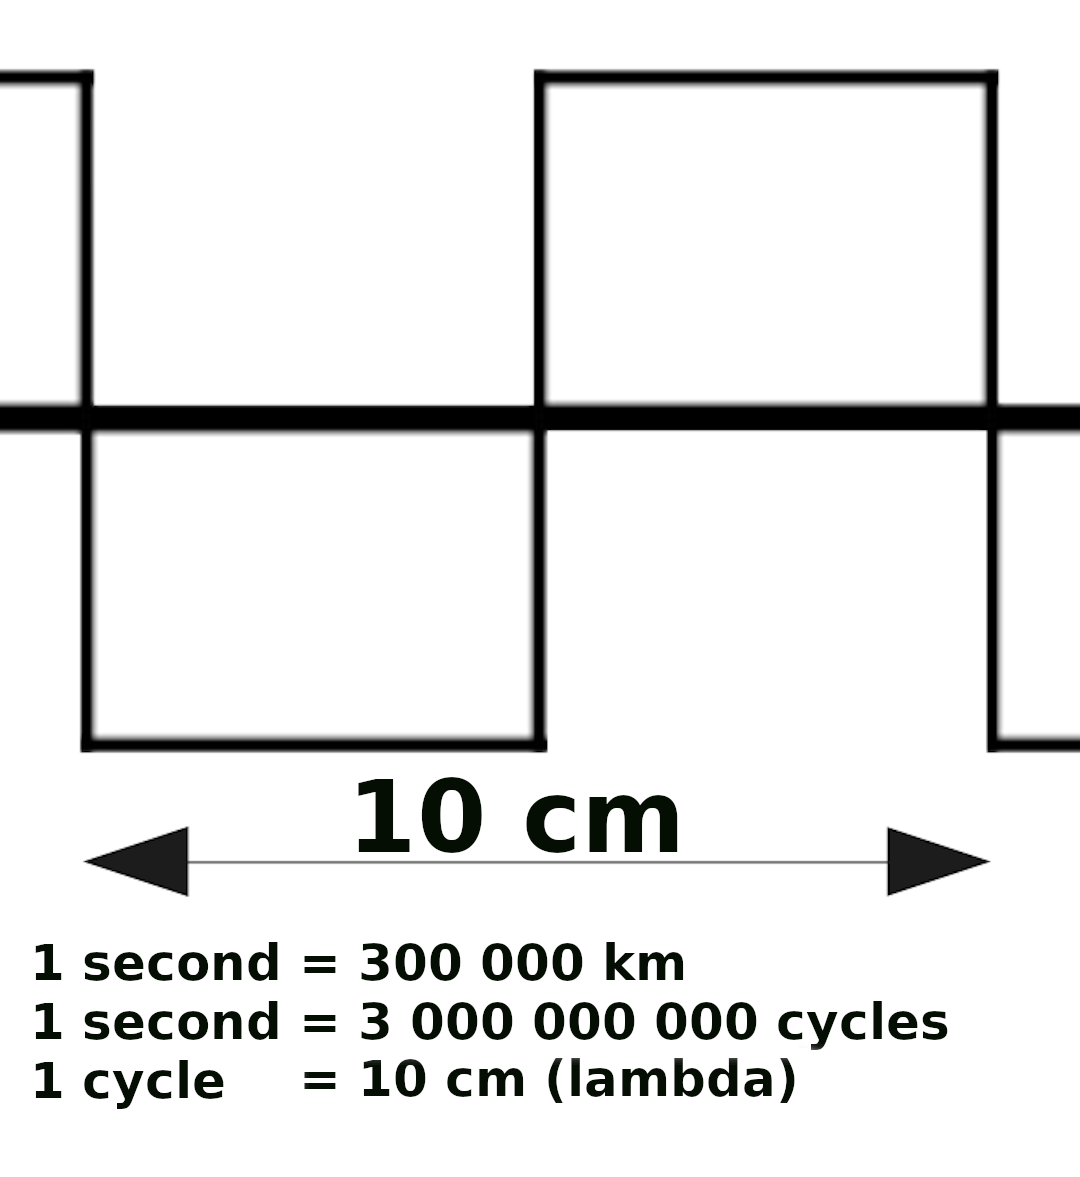
\includegraphics[width=0.50\linewidth]{os-wave3}
\caption{What is the length of a 3 GHz signal?}
\end{figure}
\end{frame}

% XXXXXXXXXXXXXXXXXXXXXXXXXXXXXXXXXXXXXXXXXXXXXXXXXXXXXXXXXXXXXXXXXXXXXXXXXX
\begin{frame}
\frametitle{Physics 101: Safe Distance for 3 GHz}
\begin{figure}
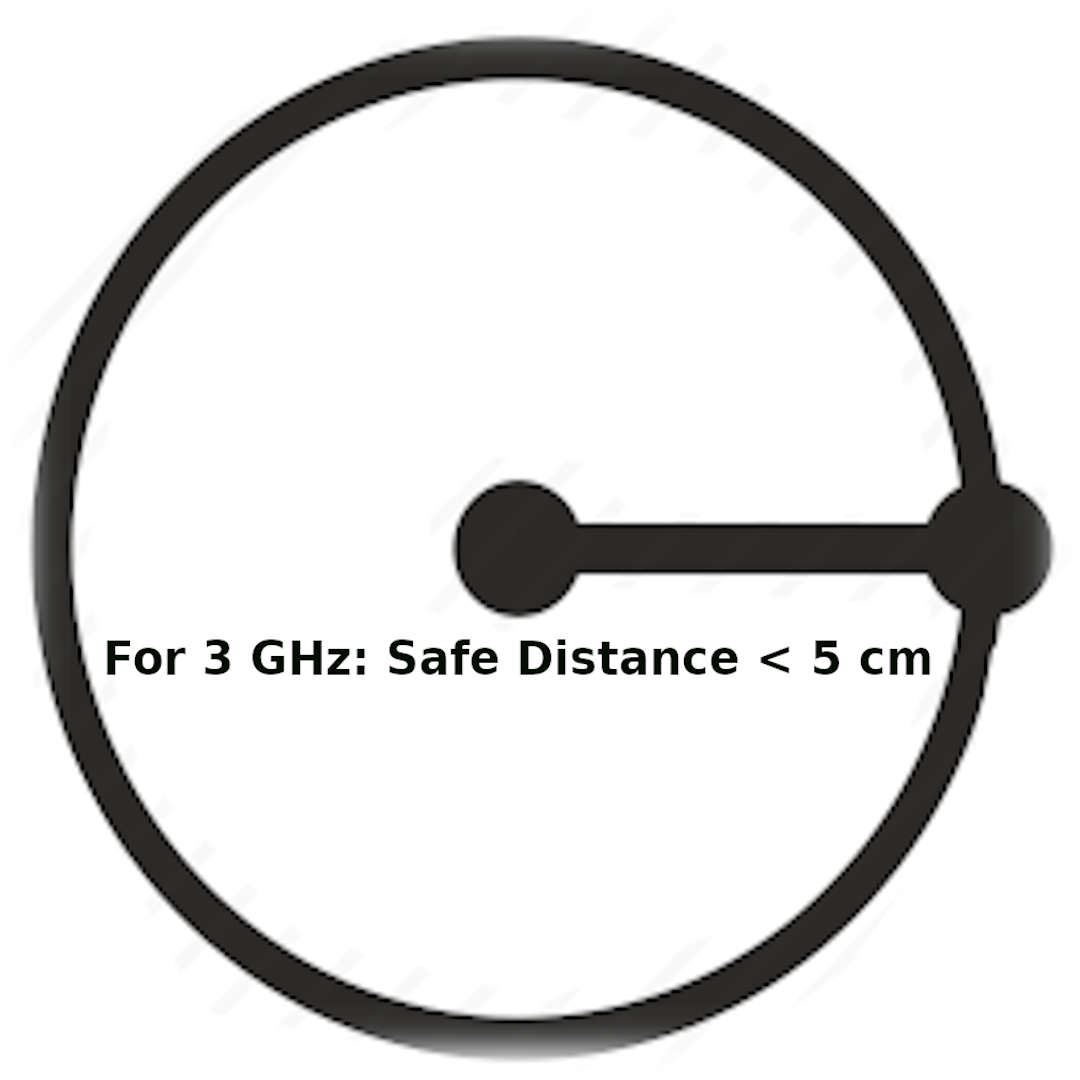
\includegraphics[width=0.50\linewidth]{os-circle}
\caption{Safe Distance}
\end{figure}
\end{frame}

% XXXXXXXXXXXXXXXXXXXXXXXXXXXXXXXXXXXXXXXXXXXXXXXXXXXXXXXXXXXXXXXXXXXXXXXXXX
\begin{frame}
\frametitle{Physics 101: Serial vs. Parallel Transmission}
\begin{figure}
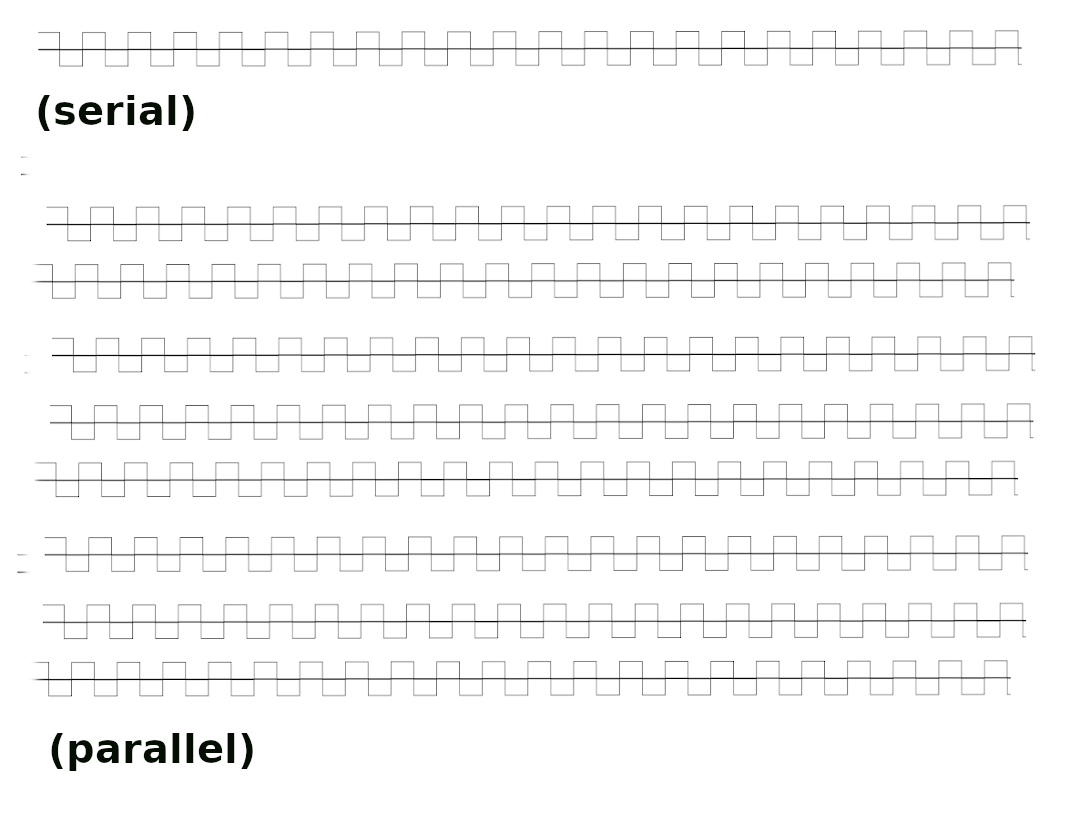
\includegraphics[width=0.65\linewidth]{os-wave4}
\caption{Serial vs. Parallel Transmission}
\end{figure}
\begin{itemize}
\item Serial: Longer Distance, easy to implement.
\item Parallel: Faster, but not easy.
\end{itemize}
\end{frame}

% XXXXXXXXXXXXXXXXXXXXXXXXXXXXXXXXXXXXXXXXXXXXXXXXXXXXXXXXXXXXXXXXXXXXXXXXXX
\begin{frame}
\frametitle{Transmission Rate (E.g. \textbf{BUS}: 64 bit/133 MHz)}
\begin{figure}
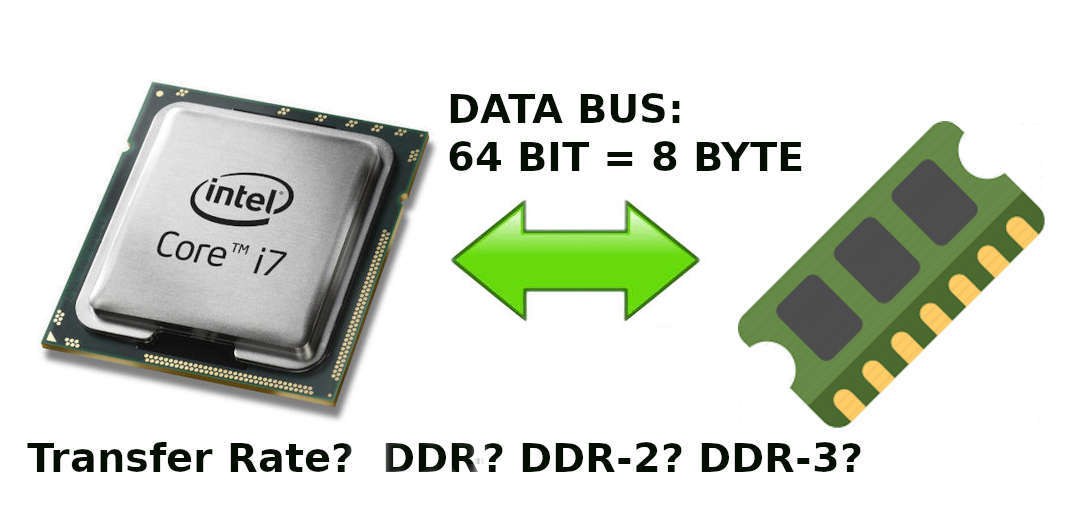
\includegraphics[width=0.61\linewidth]{os-transfer-rate}
\end{figure}
\begin{itemize}
\item E.g. \textbf{BUS}: 64 bit, \textbf{Clock}: 133 MHz
\begin{itemize}
\item SDRAM (Synchronous Dynamic RAM): 1 transmission/cycle.\\
\textbf{Transfer Rate} = \texttt{64/8 byte x 133M x 1 = 1064 Mbyte/s}.
\item DDR (Double Date Rate): 2 transmission/cycle.\\
\textbf{Transfer Rate} = \texttt{64/8 byte x 133M x 2 = 2128 Mbyte/s}.
\item DDR-2 (Double Date Rate 2): 4 transmission/cycle.\\
\textbf{Transfer Rate} = \texttt{64/8 byte x 133M x 4 = 4256 Mbyte/s}.
\item DDR-3 (Double Date Rate 3): 8 transmission per cycle.\\
\textbf{Transfer Rate} = \texttt{64/8 byte x 133M x 8 = 8512 Mbyte/s}.
\item DDR-4 = DDR-3 with a better clock rate.
\end{itemize}
\end{itemize}
\end{frame}

% XXXXXXXXXXXXXXXXXXXXXXXXXXXXXXXXXXXXXXXXXXXXXXXXXXXXXXXXXXXXXXXXXXXXXXXXXX
\begin{frame}
\frametitle{CPU: SuperVisor Mode}
\begin{figure}
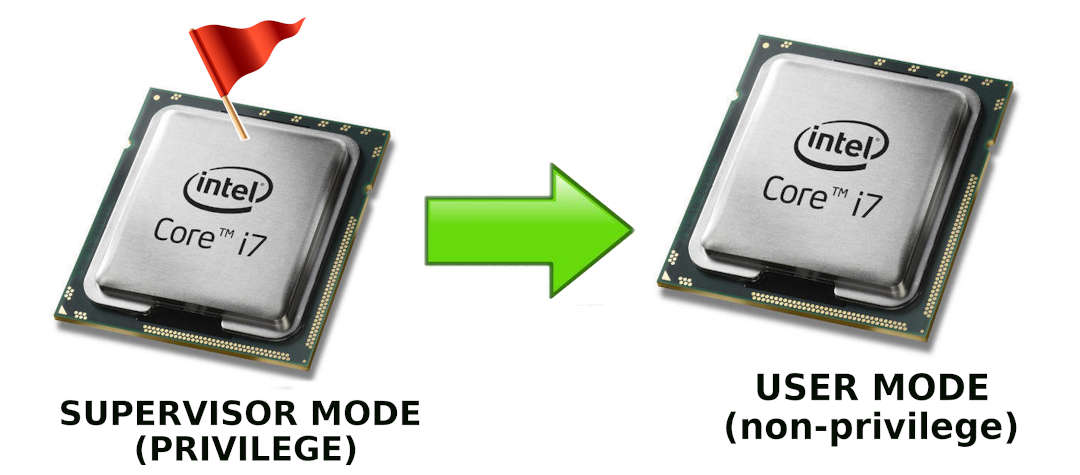
\includegraphics[width=0.65\linewidth]{os-super2user}
\caption{SuperVisor (Privilege) Mode to User Mode}
\end{figure}
\begin{itemize}
\item SuperVisor Mode
\begin{itemize}
\item A.k.a. Kernel Mode, Privilege Mode.
\item Initial STATE (Mode) of a CPU (Power On).
\item STATE (Mode) after Interrupt.
\item All operations are allowed, including to switch to User Mode!
\end{itemize}
\end{itemize}
\end{frame}

% XXXXXXXXXXXXXXXXXXXXXXXXXXXXXXXXXXXXXXXXXXXXXXXXXXXXXXXXXXXXXXXXXXXXXXXXXX
\begin{frame}
\frametitle{CPU: User Mode}
\begin{figure}
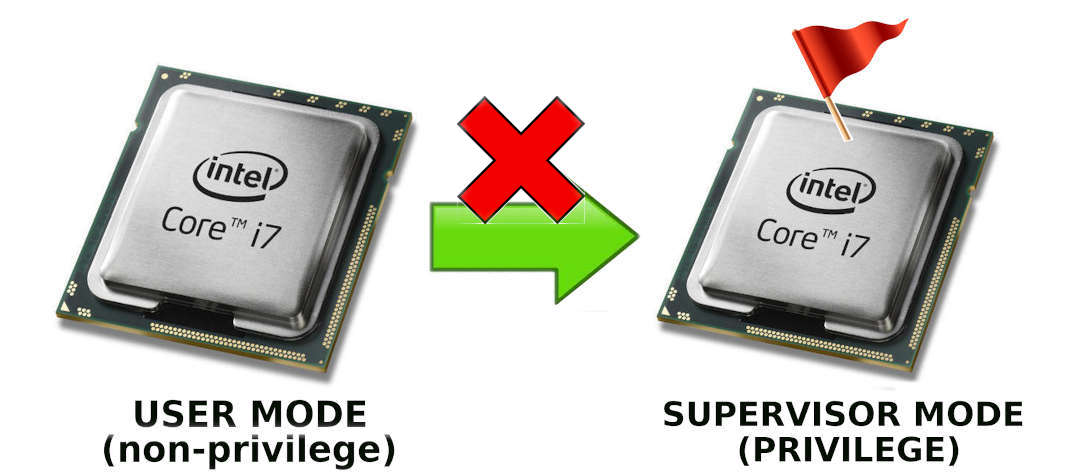
\includegraphics[width=0.65\linewidth]{os-user2super}
\caption{User Mode to SuperVisor (Privilege)}
\end{figure}
\begin{itemize}
\item User Mode
\begin{itemize}
\item It is not allowed to switch back to SuperVisor Mode.
\item It is not allowed to access I/O directly.
\item It is not allowed to modify the Interrupt Vector.
\item It is allowed to request Interrupt.
\end{itemize}
\end{itemize}
\end{frame}

% XXXXXXXXXXXXXXXXXXXXXXXXXXXXXXXXXXXXXXXXXXXXXXXXXXXXXXXXXXXXXXXXXXXXXXXXXX
\begin{frame}
\frametitle{Can you read a Block Diagram?}
\begin{figure}
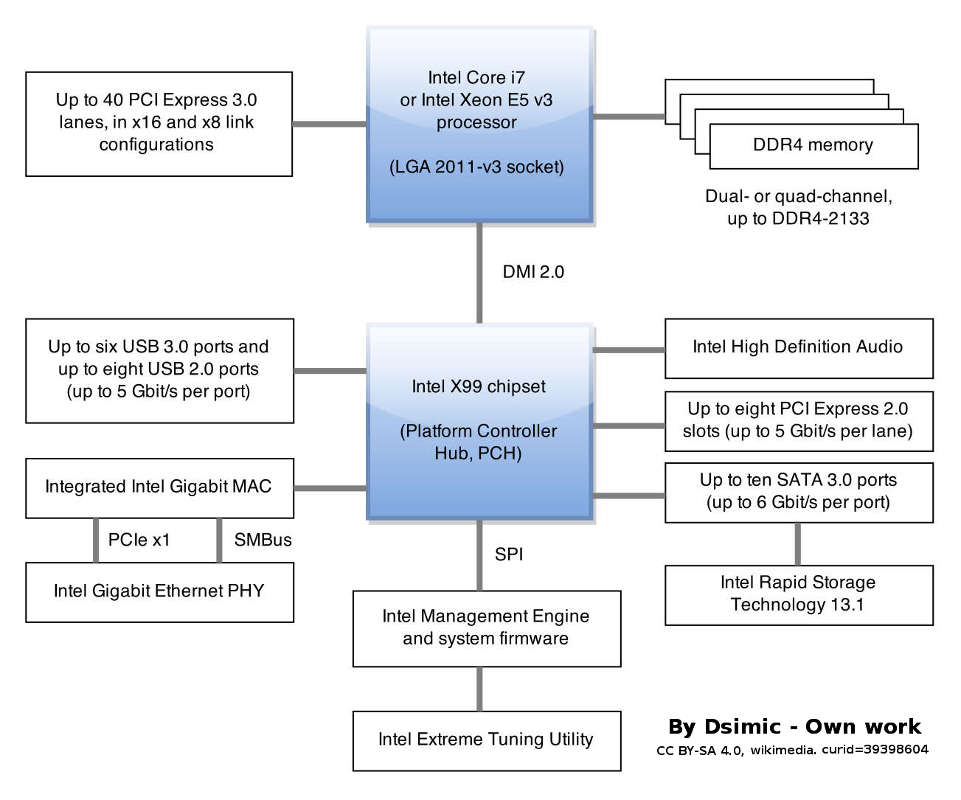
\includegraphics[width=0.70\linewidth]{os00-x99-chipset-block-diagram}
\caption{Block Diagram}
\end{figure}
\end{frame}

% XXXXXXXXXXXXXXXXXXXXXXXXXXXXXXXXXXXXXXXXXXXXXXXXXXXXXXXXXXXXXXXXXXXXXXXXXX
\begin{frame}
\frametitle{What is an APIC?!}
\begin{figure}
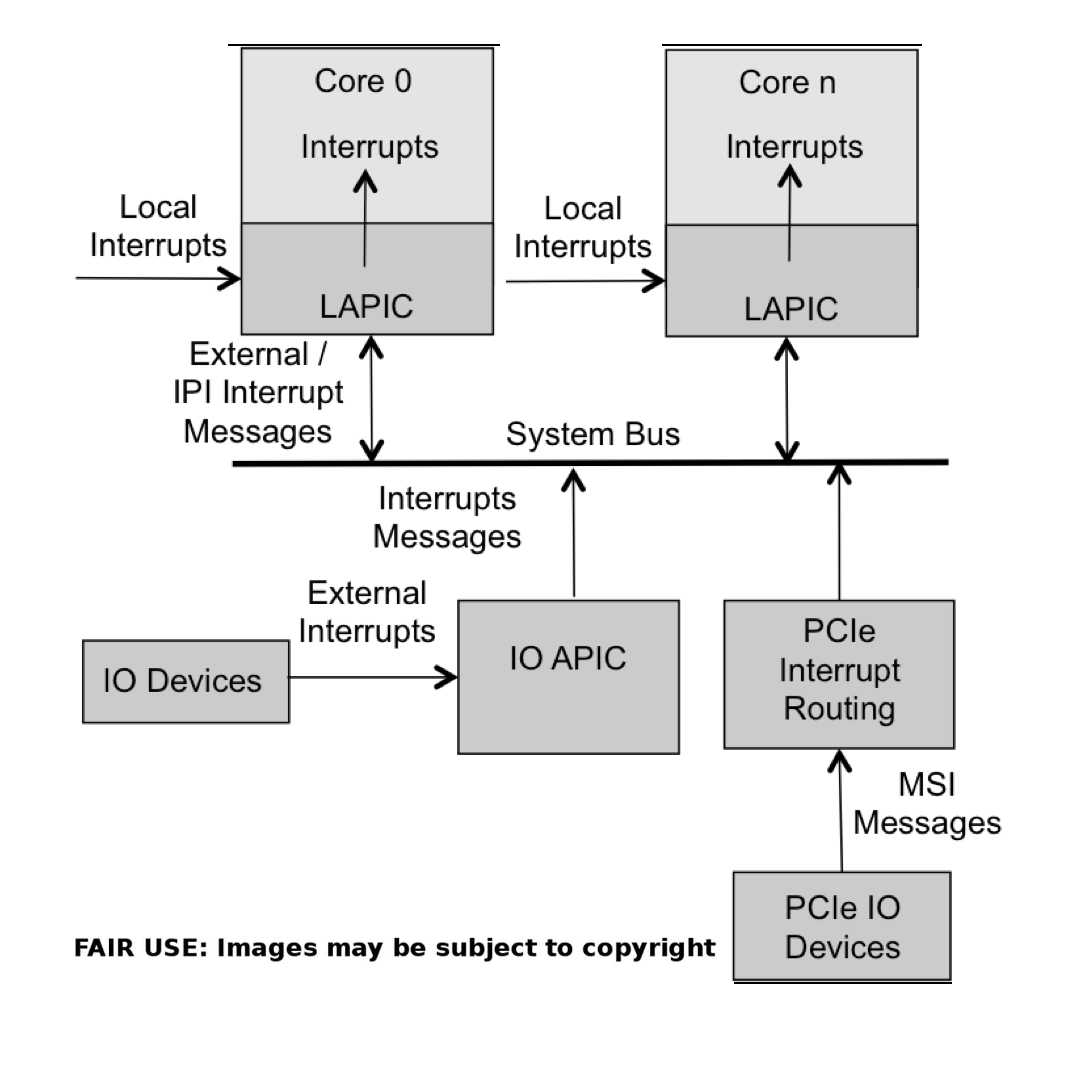
\includegraphics[width=0.60\linewidth]{os00-xapic}
\caption{APIC (Advanced Programmable Interrupt Controller)}
\end{figure}
\end{frame}

% XXXXXXXXXXXXXXXXXXXXXXXXXXXXXXXXXXXXXXXXXXXXXXXXXXXXXXXXXXXXXXXXXXXXXXXXXX
\begin{frame}
\frametitle{And, what is ''Interrupt Handling''?}
\begin{figure}
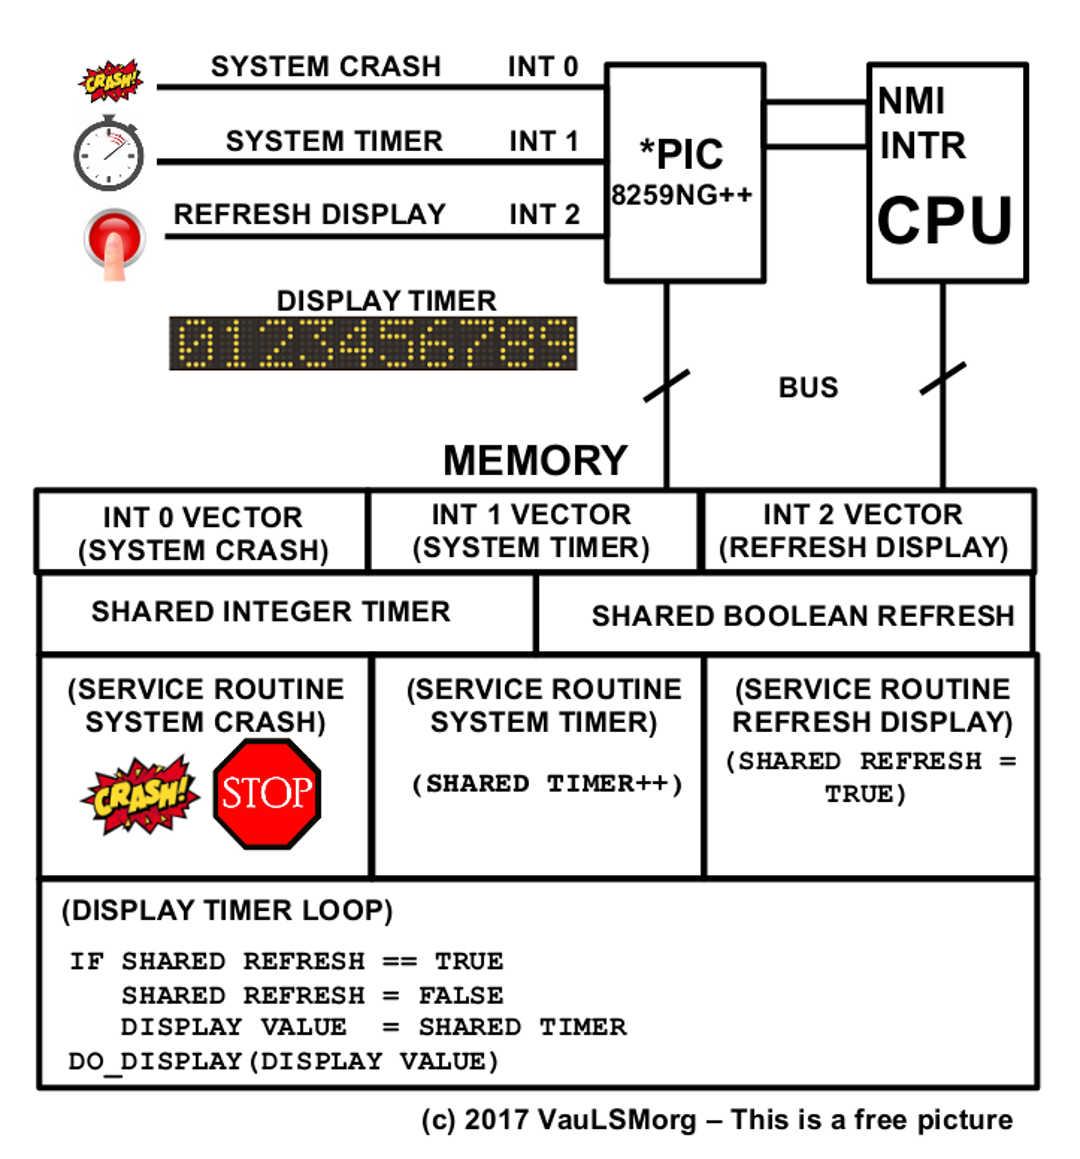
\includegraphics[width=0.56\linewidth]{os00-int-protection}
\caption{Interrupt Handling with PIC (Programmable Interrupt Controller)}
\end{figure}
\end{frame}

% XXXXXXXXXXXXXXXXXXXXXXXXXXXXXXXXXXXXXXXXXXXXXXXXXXXXXXXXXXXXXXXXXXXXXXXXXX
\begin{frame}
\frametitle{The Operating System Managers}
\begin{itemize}
\item Process Manager: 
\begin{itemize}
\item Creating/Deleting; Suspending/Resuming; Synchronization; Communication; Scheduling
\end{itemize}
\item Memory Manager:
\begin{itemize}
\item Tracking; Move In/Move Out; Allocating/Deallocating.
\end{itemize}
\item Storage/File System Manager:
\begin{itemize}
\item Create/Delete; Open/Close; Read/Write.
\end{itemize}
\item Mass Storage Manager:
\begin{itemize}
\item Scheduling; Allocating; Free Space.
\end{itemize}
\item I/O Manager:
\begin{itemize}
\item Buffering; Caching; Spooling.
\item Interfacing (driving).
\end{itemize}
\item Protecting \& Security Manager:
\begin{itemize}
\item Protecting.
\item Security.
\end{itemize}
\end{itemize}
\end{frame}

% XXXXXXXXXXXXXXXXXXXXXXXXXXXXXXXXXXXXXXXXXXXXXXXXXXXXXXXXXXXXXXXXXXXXXXXXXX
\begin{frame}
\frametitle{Any idea what these following terms mean?!}
\begin{itemize}
\item Scripting: bash, regex, sed, awk
\item Security and Protection
\item File System
\item Data Structure in a (logical) Memory
\item Virtual Memory
\item Concurrency
\item Synchronization
\item Mass Storage
\item UEFI, GRUB, and systemd
\item I/O
\item I/O Programming
\end{itemize}
\end{frame}

% XXXXXXXXXXXXXXXXXXXXXXXXXXXXXXXXXXXXXXXXXXXXXXXXXXXXXXXXXXXXXXXXXXXXXXXXXX
\begin{frame}
\frametitle{Week 00: QUIZ Example \#1 (from OSC2e)}
\begin{figure}
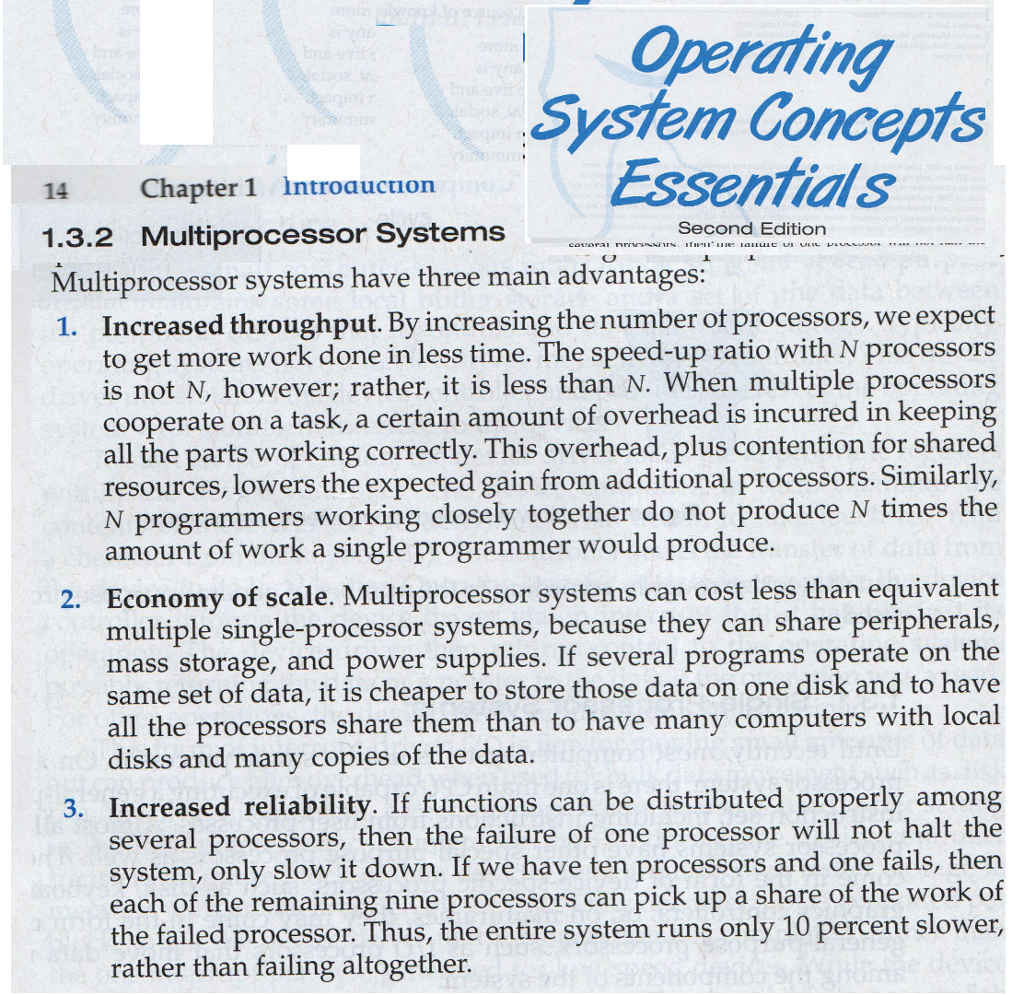
\includegraphics[width=0.56\linewidth]{os00-osc2e}
\caption{\textbf{T / F} The advantages of a multiprocessor system include: 
increased throughput, economy of scale, and increased reliability 
(Week 00 2016-1).}
\end{figure}
\end{frame}

% XXXXXXXXXXXXXXXXXXXXXXXXXXXXXXXXXXXXXXXXXXXXXXXXXXXXXXXXXXXXXXXXXXXXXXXXXX
\begin{frame}
\frametitle{Week 00: More QUIZ Examples}
\begin{itemize}
\item \textbf{TRUE/FALSE}\\
      The best way to get any help is to send an email to \texttt{operatingsystems@vlsm.org}.
\item \textbf{TRUE/FALSE}\\
      Questions regarding assignments should be posted at SCELE.
\item \textbf{TRUE/FALSE}\\
      Making a \textbf{PUSS IN BOOT} face is increasing the chance to get a better deal.
\item \textbf{TRUE/FALSE}\\
      Anyone can appeal any time, even after the (official) final grade is announced on SIAK.
\item \textbf{TRUE/FALSE}\\
      There are bonus points for early assignment submission.
\end{itemize}
\end{frame}

% XXXXXXXXXXXXXXXXXXXXXXXXXXXXXXXXXXXXXXXXXXXXXXXXXXXXXXXXXXXXXXXXXXXXXXXXXX
\section{Assignments}
\begin{frame}[fragile]
\frametitle{Assignments}
\begin{itemize}
\item There will be no mid-term (UTS) nor final-term (UAS). 
      Instead, there will be 11 weekly assignments.
      Your grade will be taken from the best 9 out of 11 assignments.
\item You need to run ''VirtualBox'' on a computer with more than 4GB RAM and up to 100 GB disk space.
\item Each assignment deadline will be by the end of that ''week''. 
      The weekly schedule will always be on the page \textbf{[\pageref{laman}]}.
\item Use the \textbf{''GitHub web interface''} for the Week 00 assignment.
      However, starting Week 01, you need to understand \textbf{''pull, add, commit, push, and ssh-keys''}.
\item Submit (push) the assignments to \url{https://github.com/}.
      If you still don't have one, you need to sign up for a \url{https://github.com/} account.
      More information will follow.
\item There will be a ''checklist'' at the end of this presentation.
\item By popular demand, the weekly schedule will be repeated on the following page!
\end{itemize}
\end{frame}

% XXXXXXXXXXXXXXXXXXXXXXXXXXXXXXXXXXXXXXXXXXXXXXXXXXXXXXXXXXXXXXXXXXXXXXXXXX

%%%%%%%%%%%%%%%%%%%%%%%%%%%%%%%%%%%%%%%%%%%%%%%%%%%%%%%%%%%%%%%%%%%%%%%%%
% REV352 Sun 10 Oct 2021 09:56:47 WIB
% REV341 Sun 05 Sep 2021 23:30:00 WIB
% REV333 Thu 26 Aug 2021 08:52:24 WIB
% REV328 Sat 14 Aug 2021 06:32:08 WIB
% REV272 Mon 01 Mar 2021 12:02:09 WIB
% START0 Sat Sep  2 10:51:33 WIB 2017
%%%%%%%%%%%%%%%%%%%%%%%%%%%%%%%%%%%%%%%%%%%%%%%%%%%%%%%%%%%%%%%%%%%%%%%%%

\begin{frame}[fragile]
\section{Schedule}
\frametitle{OS212\footnote{%
) This information will be on \textbf{EVERY} page two (2) of this course material.}): 
Operating Systems 2021 - 2}
\scalebox{0.73}{%
\begin{tabular}{|c|c|c|c|}
\hline
\makebox[106pt]{OS A} & \makebox[106pt]{OS B} & \makebox[107pt]{OS C} & \makebox[107pt]{OS INT} \\
\hline
\multicolumn{4}{|c|}{Every first day of the Week, \textbf{Quiz\#1:} (07:40-07:50) and \textbf{Quiz\#2:} 07:20-07:40} \\
\hline
Monday/Thursday & Monday/Thursday & Monday/Thursday & Monday/Wednesday   \\
13:00 --- 14:40  & 15:00 --- 16:40\footnote{) \textbf{OS B:} Week00-Week05 (RMS); Week06-Week10 (MAM).} &
                                      13:00 --- 14:40 & 08:00 --- 09:40  \\
14:00 --- finish & 16:00 --- finish & 13:00 --- 14:40 & 09:00 --- finish \\
\hline
\end{tabular}
}

\vspace{5pt}

\scalebox{0.73}{%
\begin{tabular}{|c|c|l|l|}
\hline
\textbf{Week} & \textbf{Schedule \& Deadline}\footnote{%
    ) The \textbf{DEADLINE} of Week 00 is 05 Sep 2021,
      whereas the \textbf{DEADLINE} of Week 01 is 12 Sep 2021, and so on...%
    })& \textbf{Topic} & \textbf{OSC10}\footnote{%
    ) Silberschatz et. al.: \textbf{Operating System Concepts}, $10^{th}$ Edition, 2018.}) \\
\hline
Week 00  & 30 Aug - 05 Sep 2021 & Overview 1, Virtualization \& Scripting & Ch. 1, 2, 18. \\
Week 01  & 06 Sep - 12 Sep 2021 & Overview 2, Virtualization \& Scripting & Ch. 1, 2, 18. \\
Week 02  & 13 Sep - 19 Sep 2021 & Security, Protection, Privacy, \& C-language.  & Ch. 16, 17. \\
Week 03  & 20 Sep - 26 Sep 2021 & File System \& FUSE  & Ch. 13, 14, 15. \\
Week 04  & 27 Sep - 03 Oct 2021 & Addressing, Shared Lib, \& Pointer & Ch. 9. \\
Week 05  & 04 Oct - 10 Oct 2021 & Virtual Memory & Ch. 10. \\
\hline
Week 06  & 11 Oct - 31 Oct 2021 & Concurrency: Processes \& Threads & Ch. 3, 4. \\
Week 07  & 01 Nov - 07 Nov 2021 & Synchronization \& Deadlock & Ch. 6, 7, 8. \\
Week 08  & 08 Nov - 14 Nov 2021 & Scheduling + W06/W07 & Ch. 5. \\
Week 09  & 15 Nov - 21 Nov 2021 & Storage, Firmware, Bootloader, \& Systemd & Ch. 11. \\
Week 10  & 22 Nov - 28 Nov 2021 & I/O \& Programming & Ch. 12. \\%
% MidTerm  & 00 XXX 2020 (XX:XX-XX:XX) & MidTerm (UTS) & \cellcolor{red!44} TBA! \\
% Reserved & 00 XXX - 00 XXX 2020 & Q \& A & \\
% Final    & 00 XXX 2020 XX:XX & First Part Final  (UAS tahap I)  & \cellcolor{red!44} This schedule is   \\
% Extra    & NA & No Extra assignment & \cellcolor{red!44} subject to change. \\
\hline
\end{tabular}
}
\end{frame}

\begin{frame}[fragile]
\frametitle{\textbf{STARTING POINT} --- 
{
\definecolor{links}{HTML}{FDEE00}
\hypersetup{colorlinks,linkcolor=,urlcolor=links}
\url{https://os.vlsm.org/}
}
}
\begin{itemize}
\item[$\square$] \textbf{Text Book} ---
                 Any recent/decent OS book. Eg. (\textbf{OSC10}) Silberschatz et. al.: 
                 \textbf{Operating System Concepts}, $10^{th}$ Edition, 2018.
                 See also \url{https://www.os-book.com/OS10/}.
\item[$\square$] \textbf{Resources}
\begin{itemize}
\item[$\square$] \href{https://scele.cs.ui.ac.id/course/view.php?id=3268}{\textbf{SCELE OS212}} ---
\url{https://scele.cs.ui.ac.id/course/view.php?id=3268}.\\
The enrollment key is \textbf{XXX}.
\item[$\square$] \textbf{Download Slides and Demos from GitHub.com} \\
\url{https://github.com/UI-FASILKOM-OS/SistemOperasi/}:

                 {\scriptsize%
                 \href{https://os.vlsm.org/Slides/os00.pdf}{\texttt{os00.pdf} (W00)},
                 \href{https://os.vlsm.org/Slides/os01.pdf}{\texttt{os01.pdf} (W01)},
                 \href{https://os.vlsm.org/Slides/os02.pdf}{\texttt{os02.pdf} (W02)},
                 \href{https://os.vlsm.org/Slides/os03.pdf}{\texttt{os03.pdf} (W03)},

                 \href{https://os.vlsm.org/Slides/os04.pdf}{\texttt{os04.pdf} (W04)},
                 \href{https://os.vlsm.org/Slides/os05.pdf}{\texttt{os05.pdf} (W05)},
                 \href{https://os.vlsm.org/Slides/os06.pdf}{\texttt{os06.pdf} (W06)},
                 \href{https://os.vlsm.org/Slides/os07.pdf}{\texttt{os07.pdf} (W07)},

                 \href{https://os.vlsm.org/Slides/os08.pdf}{\texttt{os08.pdf} (W08)},
                 \href{https://os.vlsm.org/Slides/os09.pdf}{\texttt{os09.pdf} (W09)},
                 \href{https://os.vlsm.org/Slides/os10.pdf}{\texttt{os10.pdf} (W10)}.
                 }
\item[$\square$] \textbf{Problems}\\
                 {\scriptsize% 
                 \href{https://rms46.vlsm.org/2/195.pdf}{\texttt{195.pdf} (W00)},
                 \href{https://rms46.vlsm.org/2/196.pdf}{\texttt{196.pdf} (W01)},
                 \href{https://rms46.vlsm.org/2/197.pdf}{\texttt{197.pdf} (W02)},
                 \href{https://rms46.vlsm.org/2/198.pdf}{\texttt{198.pdf} (W03)},\\
                 \href{https://rms46.vlsm.org/2/199.pdf}{\texttt{199.pdf} (W04)},
                 \href{https://rms46.vlsm.org/2/200.pdf}{\texttt{200.pdf} (W05)},
                 \href{https://rms46.vlsm.org/2/201.pdf}{\texttt{201.pdf} (W06)},
                 \href{https://rms46.vlsm.org/2/202.pdf}{\texttt{202.pdf} (W07)},\\
                 \href{https://rms46.vlsm.org/2/203.pdf}{\texttt{203.pdf} (W08)},
                 \href{https://rms46.vlsm.org/2/204.pdf}{\texttt{204.pdf} (W09)},
                 \href{https://rms46.vlsm.org/2/205.pdf}{\texttt{205.pdf} (W10)}.}
\item[$\square$] \textbf{LFS} --- \url{http://www.linuxfromscratch.org/lfs/view/stable/}
\item[$\square$] \textbf{OSP4DISS} --- \url{https://osp4diss.vlsm.org/}
\item[$\square$] \textbf{DOIT} --- \url{https://doit.vlsm.org/001.html}
\end{itemize}
\end{itemize}
\end{frame}



% XXXXXXXXXXXXXXXXXXXXXXXXXXXXXXXXXXXXXXXXXXXXXXXXXXXXXXXXXXXXXXXXXXXXXXXXXX
\section{Week 00 Assignments}
\begin{frame}[fragile]
\frametitle{Week 00 Assignments}
\begin{itemize}
\item Assignment \#1: Public Repository
\begin{itemize}
\item \url{https://github.com/} --- Account
\end{itemize}
\item Assignment \#2: Start Week 00 Log
\begin{itemize}
\item This is a \textbf{4 UNIT(SKS) or 12 hours/week} course. Are you sure that you have only spend 5 minutes this week???
\item E.g. see cbkadal's log at \url{https://cbkadal.github.io/os212/TXT/mylog.txt}
\item For log codes, see \url{https://osp4diss.vlsm.org/ETC/logCodes.txt}
\end{itemize}
\item Assignment \#3: Create Your GitHub Page
\begin{itemize}
\item E.g. cbkadal's page at: \url{https://cbkadal.github.io/os212/}
\end{itemize}
\item Assignment \#4: Course Registration
\begin{itemize}
\item The Google Form link will be available at
\href{https://scele.cs.ui.ac.id/mod/forum/discuss.php?d=30285}{\textbf{SCELE}}.
\end{itemize}
\item Assignment \#5: Reading/Watching Assignments
\begin{itemize}
\item What defines an Operating System?\\ \url{https://rahmatm.samik-ibrahim.vlsm.org/2021/07/what-defines-operating-system.html}
\end{itemize}
\end{itemize}
\end{frame}


% XXXXXXXXXXXXXXXXXXXXXXXXXXXXXXXXXXXXXXXXXXXXXXXXXXXXXXXXXXXXXXXXXXXXXXXXXX

\section{Week 00 Assignment \#1: Public Repository}
\begin{frame}[fragile]
\frametitle{Week 00 Assignment \#1: Public Repository}
\begin{itemize}
\item This is neither programming nor a web course. However,
      assignments will be submitted to GitHub and will be displayed on GitHub Page. 
\item Visit \url{https://github.com}:
\begin{itemize}
\item \textbf{SIGN UP}, if you have no account: (\url{https://github.com/join}).
\begin{itemize}
\item Preferably, use all lower case characters for your GitHub account.
\end{itemize}
\item Else, \textbf{SIGN IN}: (\url{https://github.com/login}).
\end{itemize}
\item Create a new repository (or repo):
\begin{itemize}
\item \textbf{Repository name}, e.g:
\begin{itemize}
\item ''os212'' for year 2021-2 (odd  semester 2021/2022),
\item ''os221'' for year 2022-1 (even semester 2021/2022),
\item ''os222'' for year 2022-2 (odd  semester 2022/2023),
\item ''os231'' for year 2023-1 (even semester 2022/2023),
\item etc.
\item \textbf{Note}: For ''os'', use lowercase. Do not use uppercase!
\end{itemize}
\item \textbf{Description}: (e.g.) Operating Systems 2021-2 (Odd Semester 21/22).
\item \textbf{Public}: Anyone can see this repository.
\item A simple \textbf{README.md} file.
\end{itemize}
\end{itemize}

\end{frame}

% XXXXXXXXXXXXXXXXXXXXXXXXXXXXXXXXXXXXXXXXXXXXXXXXXXXXXXXXXXXXXXXXXXXXXXXXXX
\begin{frame}[fragile]
\frametitle{Week 00 Assignment \#1 (cont)}

\begin{figure}
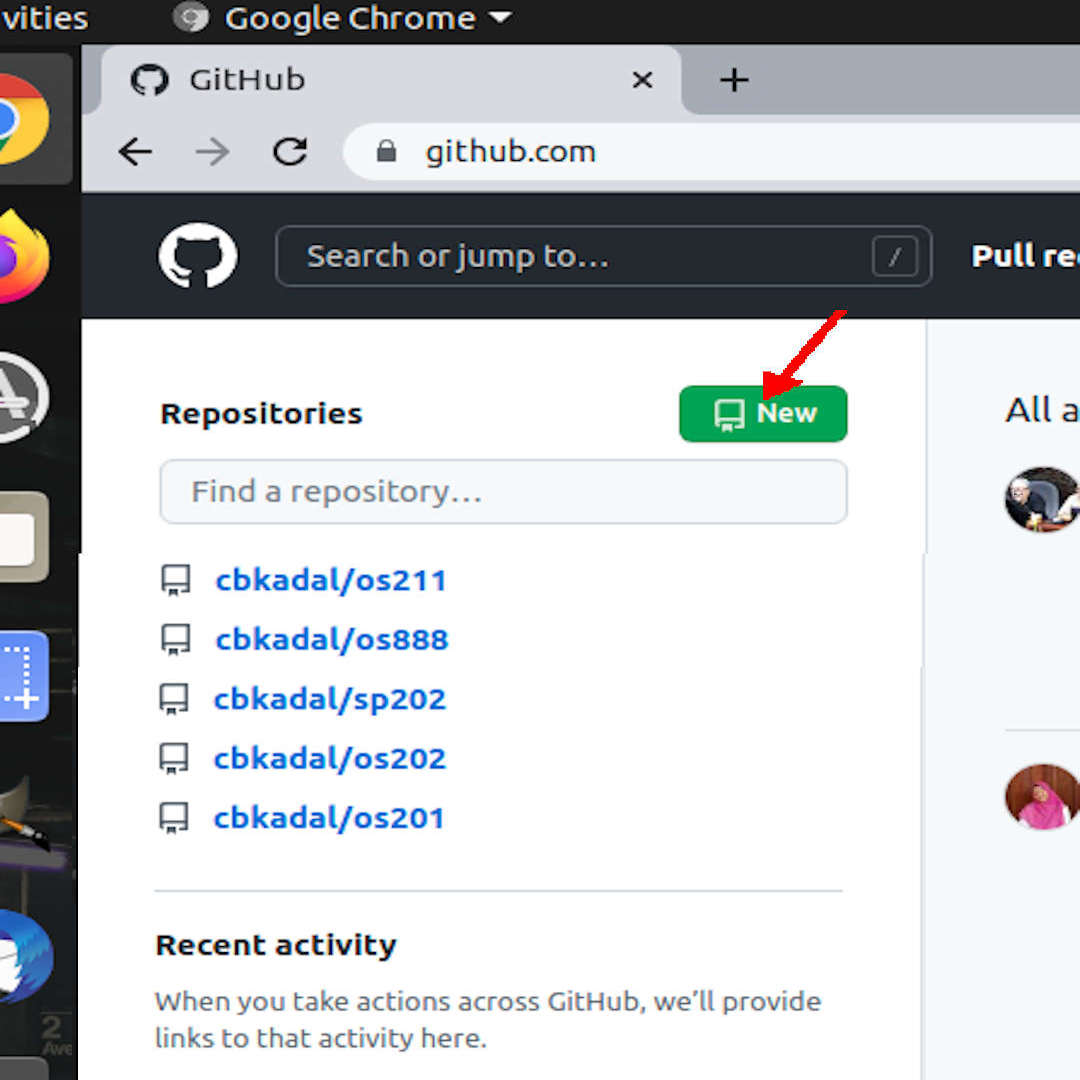
\includegraphics[width=0.60\linewidth]{os-github-new1}
\caption{Create a new repository}
\end{figure}
\end{frame}

% XXXXXXXXXXXXXXXXXXXXXXXXXXXXXXXXXXXXXXXXXXXXXXXXXXXXXXXXXXXXXXXXXXXXXXXXXX
\begin{frame}[fragile]
\frametitle{Week 00 Assignment \#2 (cont)}

\begin{figure}
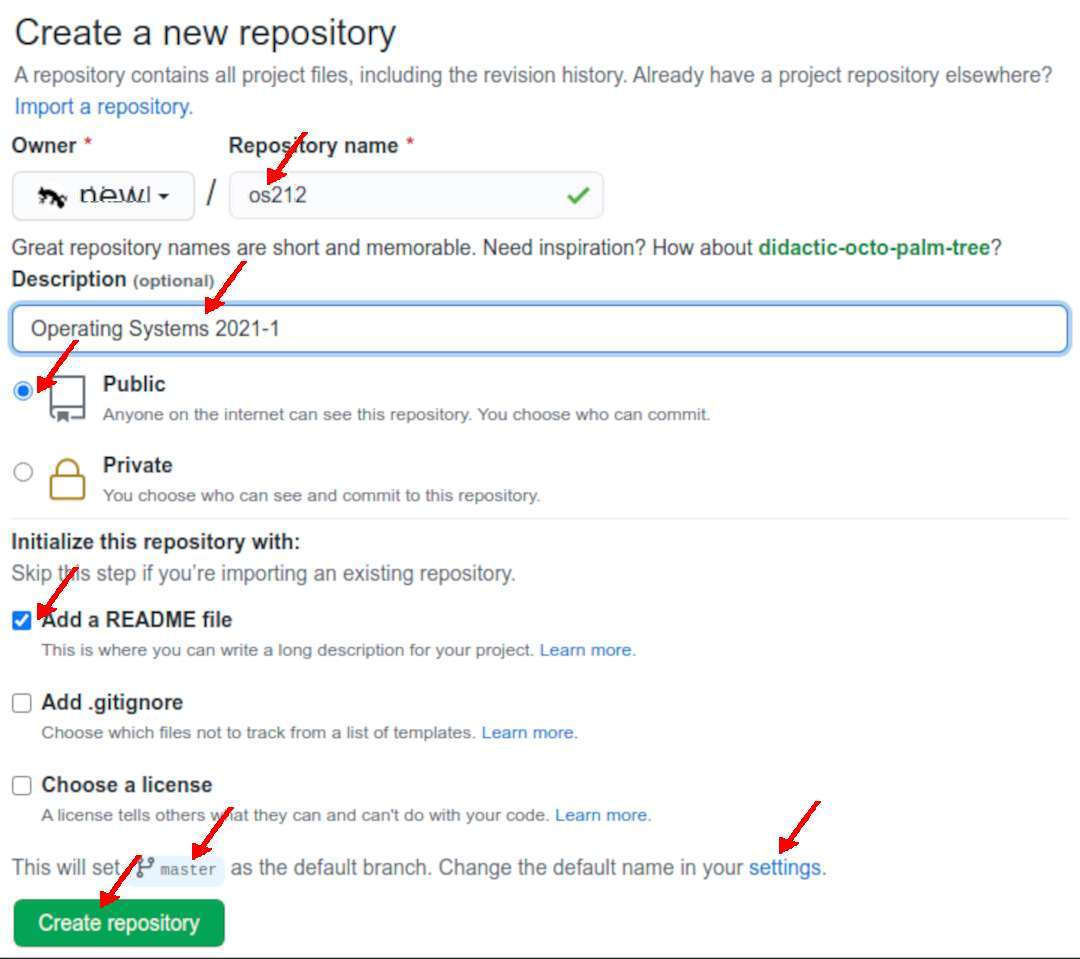
\includegraphics[width=0.69\linewidth]{os-github}
\caption{Public Repository in this example is ''os212''}
\end{figure}
\end{frame}

% XXXXXXXXXXXXXXXXXXXXXXXXXXXXXXXXXXXXXXXXXXXXXXXXXXXXXXXXXXXXXXXXXXXXXXXXXX
\begin{frame}[fragile]
\frametitle{Week 00 Assignment \#3 (cont)}
\begin{itemize}
\item The GitHub Default Branch Name Is Now ''\texttt{main}''
\begin{itemize}
\item To be "politically correct," GitHub has changed the default branch name
from ''\texttt{master}'' to ''\texttt{main}.''
\item Many past examples here have been using the ''\texttt{master}'' branch name.
      Therefore --- for being consistent --- the ''\texttt{master}'' branch name will continue to be used.
\item Feel free to use either ''\texttt{main}'' or ''\texttt{master}.'' 
      However, once it has been chosen, you should not alter your branch name.
\item To change the default branch name, click ''\texttt{settings}.''
\end{itemize}
\end{itemize}
\end{frame}

% XXXXXXXXXXXXXXXXXXXXXXXXXXXXXXXXXXXXXXXXXXXXXXXXXXXXXXXXXXXXXXXXXXXXXXXXXX
\section{Week 00 Assignment \#2: Start Week 00 Log}
\begin{frame}[fragile]
\frametitle{Week 00 Assignment \#2: Start Week 00 Log (1)}
% \large(54) \small(65) \footnotesize(72) \tiny(108) 
% \begin{lstlisting}[basicstyle=\ttfamily\large]
% \begin{lstlisting}[basicstyle=\ttfamily\small]
% \begin{lstlisting}[basicstyle=\ttfamily\footnotesize]
\begin{lstlisting}[basicstyle=\ttfamily\tiny]
# REV06 Wed 07 Jul 2021 20:15:07 WIB
# https://osp4diss.vlsm.org/ETC/logCodes.txt
# ZCZC WEEK# MINUTES LogCode Description

L00 General, etc.
L01 SCELE/Discord related
L02 ZOOM meetings related
L03 GitHub related
L04 GitHub Pages related
L05 Quiz related
L06 References/Books/Documents/GSGS related
L07 Demo related
L08 AsDos: asking, etc.
L09 Assignment in General
L10 Assignment #00
L11 Assignment #01
L12 Assignment #02
L13 Assignment #03
L14 Assignment #04
L15 Assignment #05
L16 Assignment #06
L17 Assignment #07
L18 Assignment #08
L19 Assignment #09
L20 Assignment #10
L21 Trying something
L22 Quiz
L23 Linux CLI including tar, etc.
(...)
L86 House chore, including helping mom, pap, uncle, aunty, jaga warung, jualan kue, etc.
L87 Else that is not related with this Operating Systems class.
L99 Other (...)

\end{lstlisting}
\end{frame}

% XXXXXXXXXXXXXXXXXXXXXXXXXXXXXXXXXXXXXXXXXXXXXXXXXXXXXXXXXXXXXXXXXXXXXXXXXX
\begin{frame}[fragile]
\frametitle{Week 00 Assignment \#2: (cont)}
\texttt{Add file} $\rightarrow$ \texttt{Create new file} 

      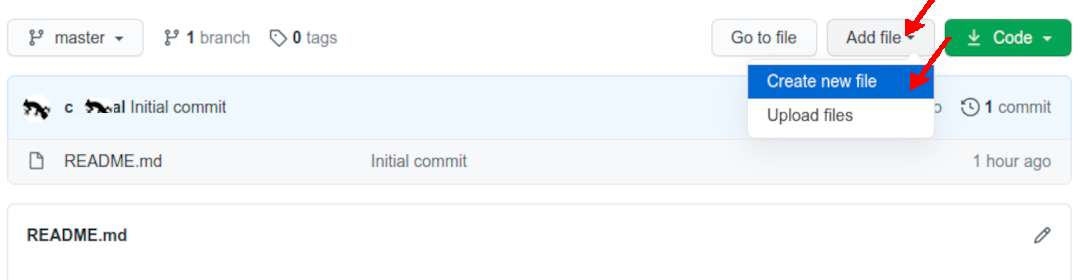
\includegraphics[width=0.65\linewidth]{os-github-new}

\textbf{Folder/File}: ''\texttt{TXT/mylog.txt}'' ({\tiny Eg. Week-00 10 minutes doing GitHub (L03)})

      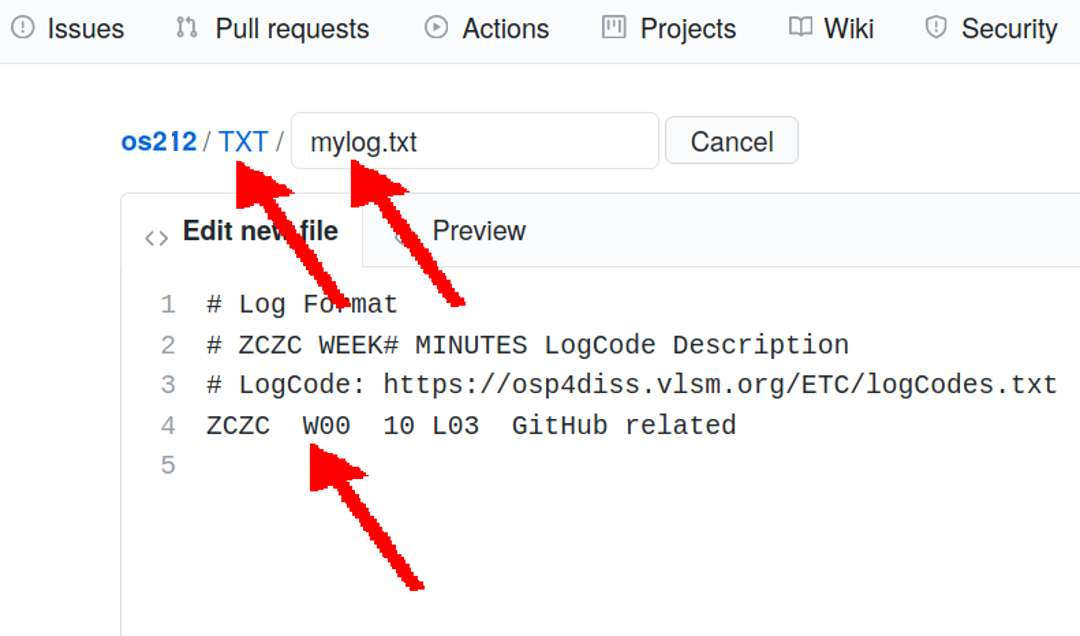
\includegraphics[width=0.65\linewidth]{os-github-file}

\end{frame}

% XXXXXXXXXXXXXXXXXXXXXXXXXXXXXXXXXXXXXXXXXXXXXXXXXXXXXXXXXXXXXXXXXXXXXXXXXX
\begin{frame}[fragile]
\frametitle{Week 00 Assignment \#2: (cont)}
Commit a new file

      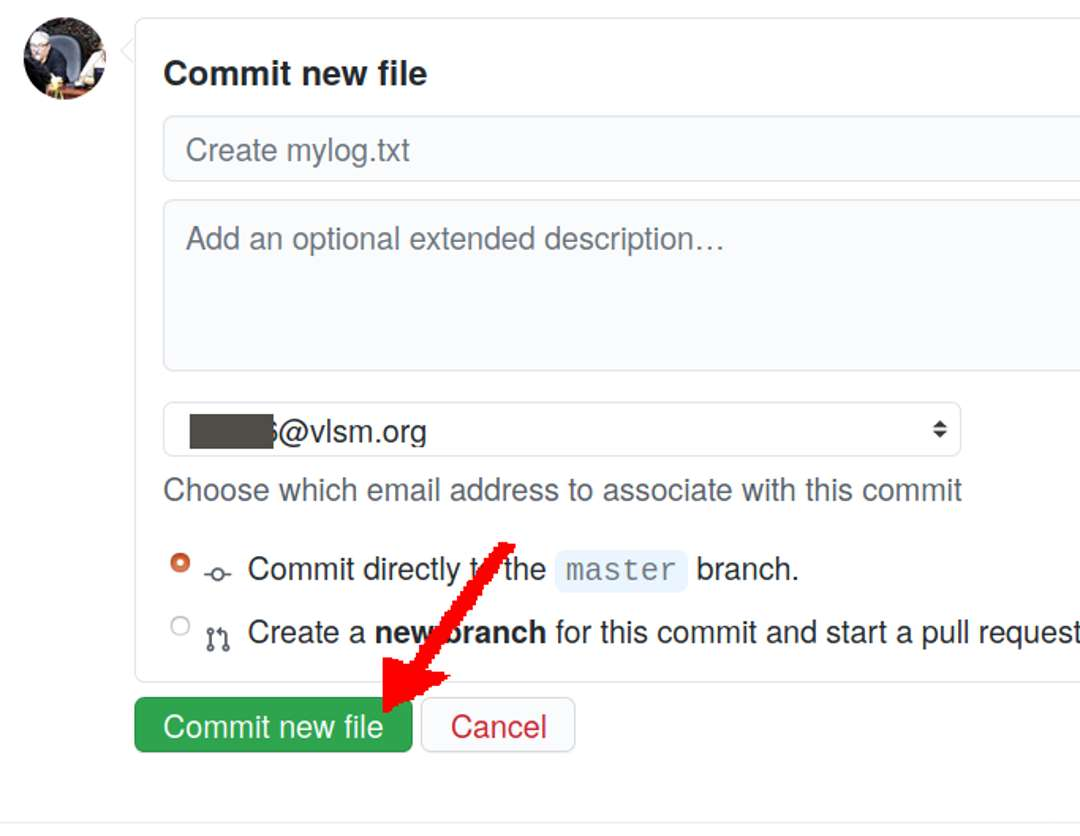
\includegraphics[width=0.80\linewidth]{os-github-commit}

\end{frame}

% XXXXXXXXXXXXXXXXXXXXXXXXXXXXXXXXXXXXXXXXXXXXXXXXXXXXXXXXXXXXXXXXXXXXXXXXXX
\section{Week 00 Assignment \#3: Create Your GitHub Page}
\begin{frame}[fragile]
\frametitle{Week 00 Assignment \#3: Create Your GitHub Page}

\begin{itemize}
\item Do GSGS\footnote{Google Sana (There) Google Sini (Here)}. 
\item Find out how to create your GitHub Page! 
E.g., if your GitHub account is ''\texttt{cbkadal}'' (Cicak Bin Kadal).
\begin{itemize}
\item The GitHub repository will be:
\begin{itemize}
\item \url{https://github.com/cbkadal/os212/}.
\end{itemize}
\item The GitHub Page will be:
\begin{itemize}
\item \url{https://cbkadal.github.io/os212/}. 
\end{itemize}
\item See also \url{https://doit.vlsm.org/001.html}
\end{itemize}
\item Your GitHub Page should be as light as possible!
\begin{itemize}
\item \textbf{The total repo size: less than 1 Mbytes}.
\item Do not apply any Jekyll theme.
\item Suggested images size: less than 50 Kbytes.
\item No external CSS and fonts.
\item Google Analytics is allowed.
\end{itemize}
\end{itemize}

\end{frame}

% XXXXXXXXXXXXXXXXXXXXXXXXXXXXXXXXXXXXXXXXXXXXXXXXXXXXXXXXXXXXXXXXXXXXXXXXXX
\section{Week 00 Assignment \#4: Course Registration}
\begin{frame}[fragile]
\frametitle{Week 00 Assignment \#4: Course Registration}

\begin{tabular}{ll}
\begin{minipage}[t]{104pt}\vspace{1pt}%

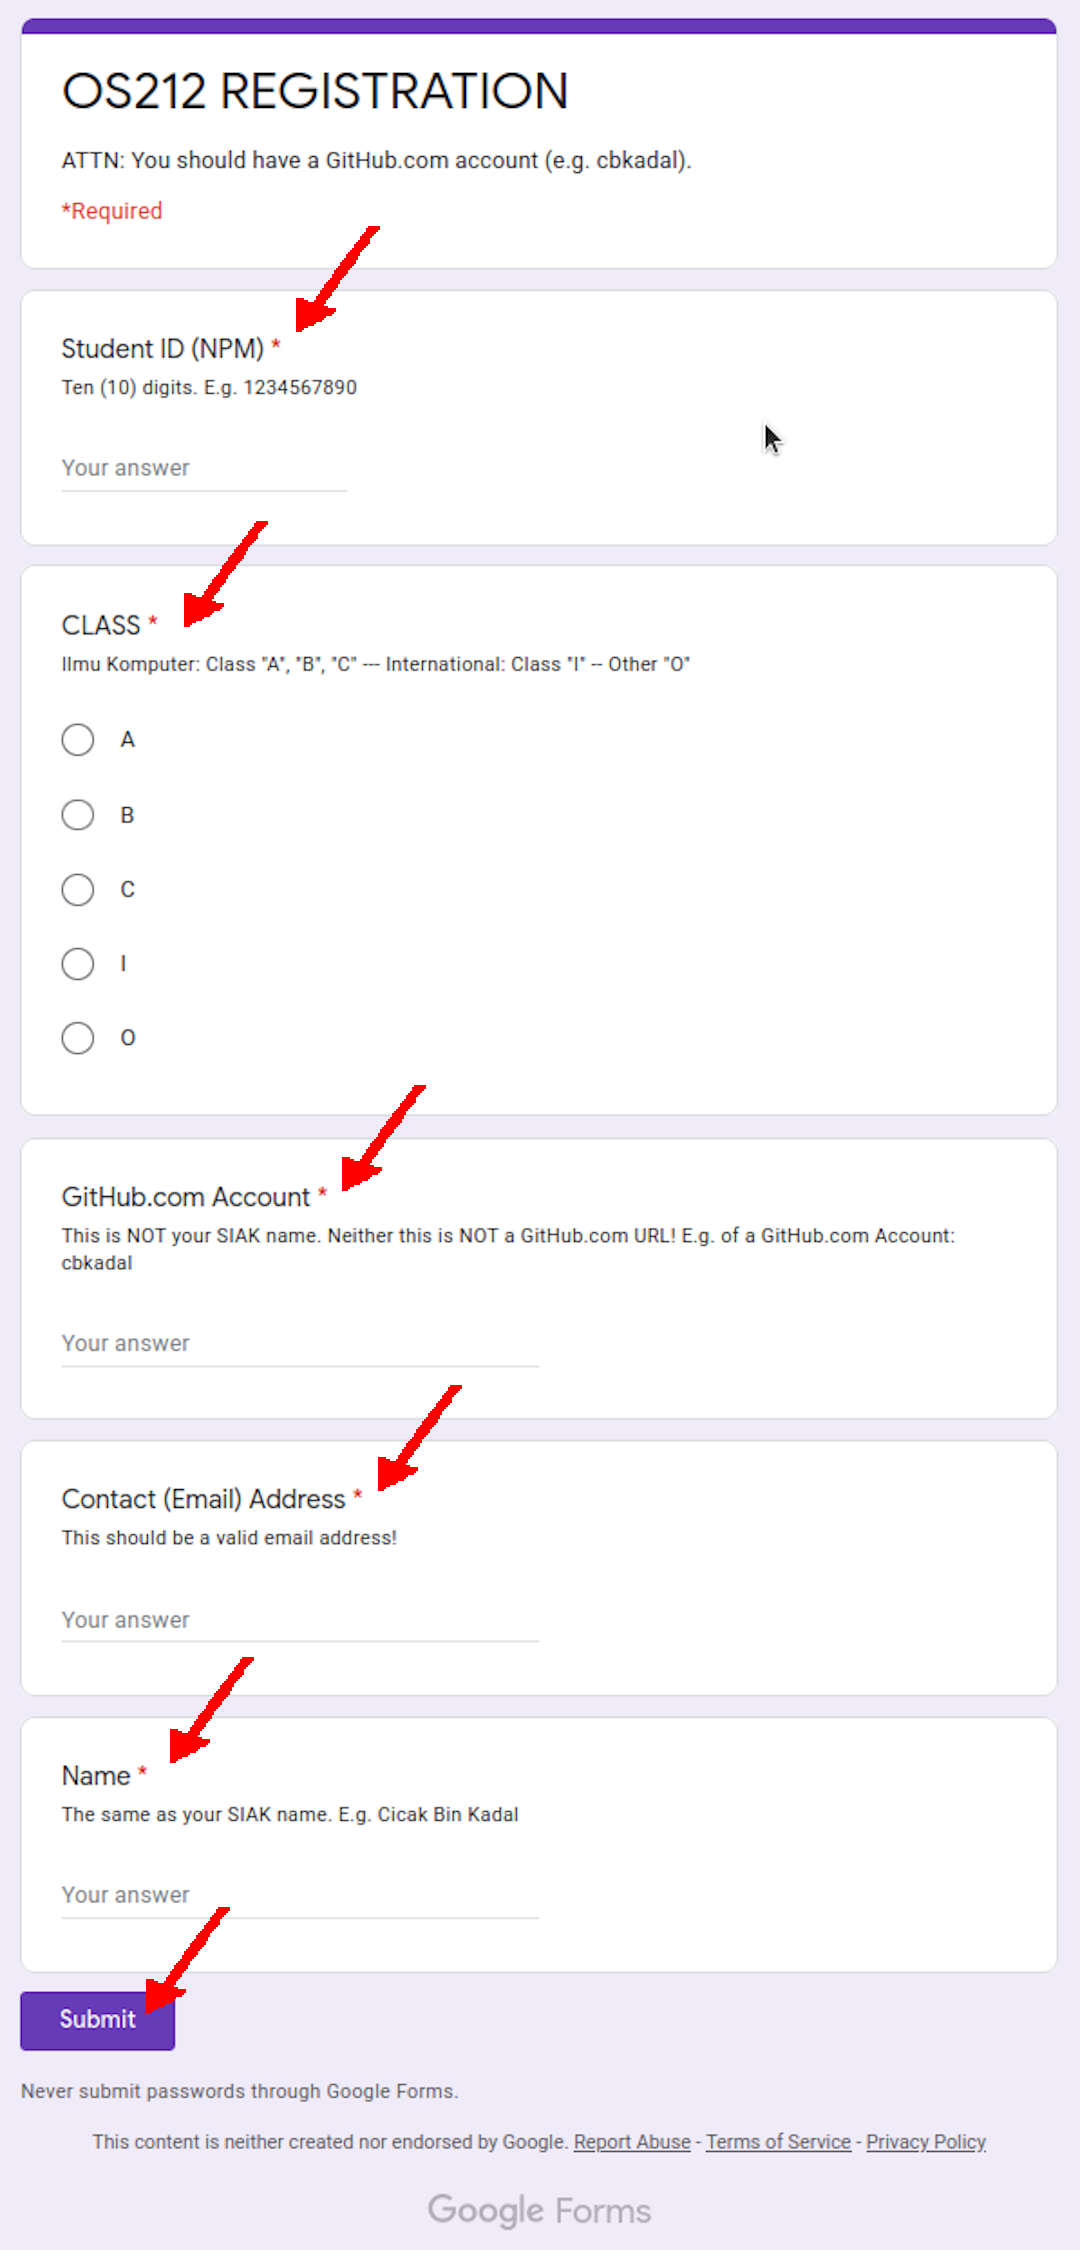
\includegraphics[width=101pt]{os-github0}

\end{minipage}%
&
\begin{minipage}[t]{224pt}\vspace{1pt}%

\begin{itemize}

\item You need a Google Account to fill this Google Form\footnote{The form content is subject to change}.

\item The Google Form link will be available at
\href{https://scele.cs.ui.ac.id/mod/forum/discuss.php?d=30285}{\textbf{SCELE}}.

\item Fill in with the email address that you normally use. It does not have to be Gmail.

\item GitHub Account example: ''\texttt{cbkadal}''.

\item ''\texttt{github.com/cbkadal/}'' \textbf{is not} a GitHub account.

\item Use your SIAK name, \textbf{NOT} your NICK name.

\item If you make a \textbf{mistake}, revisit the Google Form page.

\end{itemize}

\end{minipage}%
\\
\end{tabular}

\end{frame}

% XXXXXXXXXXXXXXXXXXXXXXXXXXXXXXXXXXXXXXXXXXXXXXXXXXXXXXXXXXXXXXXXXXXXXXXXXX
\section{Week 00 Assignment \#5: Reading/Watching Assignments}
\begin{frame}[fragile]
\frametitle{Week 00 Assignment \#5: Reading Assignment}
Get familiar with the following documents.
But, there is no need to memorize them!
\begin{itemize}
\item What defines an Operating System?\\ \url{https://rahmatm.samik-ibrahim.vlsm.org/2021/07/what-defines-operating-system.html}
\item (\textbf{OSC10}) Silberschatz et. al.:
      \textbf{Operating System Concepts}, $10^{th}$ Edition, 2018,
      \url{https://www.os-book.com/OS10/}, chapter 1, 2, 18.
\item GNU/Linux Tutorial\\ \url{https://osp4diss.vlsm.org/Welcome2GNULinux.html}
\item More GNU/Linux\\ \url{https://osp4diss.vlsm.org/osp-115.html}
\item Operating Systems: Visual Metaphor (Udacity)\\ \url{https://www.youtube.com/playlist?list=PLqoiDr4YpRdm_nzFhCDuj74P8ul5z7SdO}
\end{itemize}
\end{frame}

% XXXXXXXXXXXXXXXXXXXXXXXXXXXXXXXXXXXXXXXXXXXXXXXXXXXXXXXXXXXXXXXXXXXXXXXXXX
\section{Course Highlights and Syllabus} 
\begin{frame}
\frametitle{Course Highlights and Syllabus}
\begin{block}{Coverage}
This is an introduction to a modern operating systems course. 
It will cover
general overview,
computer architecture review,
operating system overview,
GNU/Linux CLI,
scripting,
C language overview,
protection,
security,
privacy,
systemd,
I/O,
addressing and pointers,
memory management, 
processes and threads, 
virtual memory,
synchronization,
mutual exclusion, 
deadlock, 
CPU scheduling algorithms, 
file systems,
and
I/O programming.
\end{block}

\begin{block}{Student-Centered}
This course is student-centered where responsibility is
in the hands of the students. Students are expected to 
be prepared for the class meeting.
\end{block}

\begin{block}{GNU/Linux}
Students will have a thorough understanding of how GNU/Linux 
provides services by using a Command Line Interface.
\end{block}

\end{frame}


% XXXXXXXXXXXXXXXXXXXXXXXXXXXXXXXXXXXXXXXXXXXXXXXXXXXXXXXXXXXXXXXXXXXXXXXXXX
%%%%%%%%%%%%%%%%%%%%%%%%%%%%%%%%%%%%%%%%%%%%%%%%%%%%%%%%%%%%%%%%%%%%%%%%%
% REV154 Thu Aug 23 11:22:02 WIB 2018
% START0 Thu Jul 26 20:01:45 WIB 2018
%%%%%%%%%%%%%%%%%%%%%%%%%%%%%%%%%%%%%%%%%%%%%%%%%%%%%%%%%%%%%%%%%%%%%%%%%

\section{Week 00}
\begin{frame}[fragile]
\frametitle{Week 00 Overview I:
Topics\footnote{Source: ACM IEEE CS Curricula 2013}}

\begin{itemize}
\item Role and purpose of the operating system 
\item Functionality of a typical operating system 
\item Mechanisms to support client-server models, hand-held devices 
\item Design issues (efficiency, robustness, flexibility, portability, security, compatibility) 
\item Influences of security, networking, multimedia, windowing systems 
\item Structuring methods (monolithic, layered, modular, micro-kernel models) 
\item Abstractions, processes, and resources 
\item Concepts of application program interfaces (APIs) 
\item The evolution of hardware/software techniques and application needs 
\item Device organization 
\item Interrupts: methods and implementations 
\item Concept of user/system state and protection, transition to kernel mode 
\end{itemize}
\end{frame}

\begin{frame}[fragile]
\frametitle{Week 00 Overview I:
Learning Outcomes (1)\footnote{Source: ACM IEEE CS Curricula 2013}}
\begin{itemize}
\item Explain the objectives and functions of modern operating systems [Familiarity]
\item Analyze the tradeoffs inherent in operating system design [Usage]
\item Describe the functions of a contemporary operating system with respect to convenience, efficiency, and the ability to evolve. [Familiarity] 
\item Discuss networked, client-server, distributed operating systems and how they differ from single user operating systems. [Familiarity] 
\item Identify potential threats to operating systems and the security features design to guard against them. [Familiarity] 
\item Explain the concept of a logical layer.  [Familiarity] 
\end{itemize}
\end{frame}


\begin{frame}[fragile]
\frametitle{Week 00 Overview I:
Learning Outcomes (2)\footnote{Source: ACM IEEE CS Curricula 2013}}
\begin{itemize}
\item Explain the benefits of building abstract layers in hierarchical fashion.  [Familiarity] 
\item Describe the value of APIs and middleware. [Assessment]
\item Describe how computing resources are used by application software and managed by system software.  [Familiarity] 
\item Contrast kernel and user mode in an operating system. [Usage]
\item Discuss the advantages and disadvantages of using interrupt processing. [Familiarity] 
\item Explain the use of a device list and driver I/O queue. [Familiarity] 
\end{itemize}
\end{frame}


%%%%%%%%%%%%%%%%%%%%%%%%%%%%%%%%%%%%%%%%%%%%%%%%%%%%%%%%%%%%%%%%%%%%%%%%%
% REV340 Sun 05 Sep 2021 17:25:57 WIB
% REV330 Wed 18 Aug 2021 11:05:51 WIB
% REV161 Thu Sep  6 09:24:27 WIB 2018
% REV154 Thu Aug 23 11:22:02 WIB 2018
% START0 Thu Jul 26 20:01:45 WIB 2018
%%%%%%%%%%%%%%%%%%%%%%%%%%%%%%%%%%%%%%%%%%%%%%%%%%%%%%%%%%%%%%%%%%%%%%%%%

\section{Week 01}
\begin{frame}[fragile]
\frametitle{Week 01 Overview II:
Topics\footnote{Source: ACM IEEE CS Curricula 2013}}

\begin{itemize}
\item Intelectual Property Rights (IPR)
\item Software Licenses and Free Software
\item Operating System Services and Interfaces
\item System Calls and System Programming
\item Types of virtualization (including Hardware/Software, OS, Server, Service, Network) 
\item Hypervisors 
\item Portable and cost of virtualization; emulation vs. isolation 
\item Cloud services: IAAS, PAAS and Platform APIs, SAAS
\item Introduction to Scripting and REGEX.
\end{itemize}
\end{frame}

\begin{frame}[fragile]
\frametitle{Week 01 Overview II:
Learning Outcomes\footnote{Source: ACM IEEE CS Curricula 2013}}

\begin{itemize}
\item Explain the concept of virtual memory and how it is realized in hardware and software. [Familiarity] 
\item Discuss hypervisors and the need for them in conjunction with different types of hypervisors. [Usage] 
\item Differentiate emulation and isolation. [Familiarity]
\item Evaluate virtualization trade-offs. [Assessment]
\item Discuss the importance of elasticity and resource management in cloud computing. [Familiarity]
\item Explain the advantages and disadvantages of using the virtualized infrastructure. [Familiarity]
\end{itemize}
\end{frame}


%%%%%%%%%%%%%%%%%%%%%%%%%%%%%%%%%%%%%%%%%%%%%%%%%%%%%%%%%%%%%%%%%%%%%%%%%
% REV346 Sun 12 Sep 2021 17:00:19 WIB
% REV154 Thu Aug 23 11:22:02 WIB 2018
% START0 Thu Jul 26 20:01:45 WIB 2018
%%%%%%%%%%%%%%%%%%%%%%%%%%%%%%%%%%%%%%%%%%%%%%%%%%%%%%%%%%%%%%%%%%%%%%%%%

\section{Week 02 Security \& Protection}
\begin{frame}[fragile]
\frametitle{Week 02 Security \& Protection:
Topics\footnote{Source: ACM IEEE CS Curricula 2013}}

\begin{itemize}
\item Overview of system security 
\item Cyber Security Introduction
\item Policy/mechanism separation 
\item Security methods and devices 
\item Protection, access control, and authentication 
\item Backups 
\item Safety and Privacy
\item Threads
\item Cryptography: (Symmetric and Asymmetric) Encryption,
\item C Language
\end{itemize}

\end{frame}

\begin{frame}[fragile]
\frametitle{Week 02 Security \& Protection:
Learning Outcomes\footnote{Source: ACM IEEE CS Curricula 2013}}

\begin{itemize}
\item Articulate the need for protection and security in an OS (cross-reference IAS/Security Architecture and Systems Administration/Investigating Operating Systems Security for various systems). [Assessment]
\item Summarize the features and limitations of an operating system used to provide protection and security [Familiarity] 
\item Explain the mechanisms available in an OS to control access to resources [Familiarity] 
\item Carry out simple system administration tasks according to a security policy, for example creating accounts, setting permissions, applying patches, and arranging for regular backups [Usage] 
\end{itemize}
\end{frame}


%%%%%%%%%%%%%%%%%%%%%%%%%%%%%%%%%%%%%%%%%%%%%%%%%%%%%%%%%%%%%%%%%%%%%%%%%
% REV154 Thu Aug 23 11:22:02 WIB 2018
% START0 Thu Jul 26 20:01:45 WIB 2018
%%%%%%%%%%%%%%%%%%%%%%%%%%%%%%%%%%%%%%%%%%%%%%%%%%%%%%%%%%%%%%%%%%%%%%%%%

\section{Week 03}
\begin{frame}[fragile]
\frametitle{Week 03 File System \& FUSE:
Topics\footnote{Source: ACM IEEE CS Curricula 2013}}

\begin{itemize}
\item Files: data, metadata, operations, organization, buffering, sequential, nonsequential
\item Directories: contents and structure
\item File systems: partitioning, mount/unmount, virtual file systems
\item Standard implementation techniques
\item Memory-mapped files
\item Special-purpose file systems
\item Naming, searching, access, backups
\item Journaling and log-structured file systems
\end{itemize}
\end{frame}

\begin{frame}[fragile]
\frametitle{Week 03 File System \& FUSE:
Learning Outcomes\footnote{Source: ACM IEEE CS Curricula 2013}}
\begin{itemize}
\item Describe the choices to be made in designing file systems. [Familiarity]
\item Compare and contrast different approaches to file organization, recognizing the strengths and weaknesses of each. [Usage]
\item Summarize how hardware developments have led to changes in the priorities for the design and the management of file systems. [Familiarity]
\item Summarize the use of journaling and how log-structured file systems enhance fault tolerance. [Familiarity]
\end{itemize}

\end{frame}


%%%%%%%%%%%%%%%%%%%%%%%%%%%%%%%%%%%%%%%%%%%%%%%%%%%%%%%%%%%%%%%%%%%%%%%%%
% REV349 Sun 26 Sep 2021 09:13:27 WIB
% REV154 Thu Aug 23 11:22:02 WIB 2018
% START0 Thu Jul 26 20:01:45 WIB 2018
%%%%%%%%%%%%%%%%%%%%%%%%%%%%%%%%%%%%%%%%%%%%%%%%%%%%%%%%%%%%%%%%%%%%%%%%%

\section{Week 04: Topics}
\begin{frame}[fragile]
\frametitle{Week 04 Addressing:
Topics\footnote{Source: ACM IEEE CS Curricula 2013}}

\begin{itemize}
\item Bits, bytes, and words
\item Numeric data representation and number bases
\item Representation of records and arrays
\end{itemize}
\end{frame}


\begin{frame}[fragile]
\frametitle{Week 04 Addressing:
Learning Outcomes\footnote{Source: ACM IEEE CS Curricula 2013}}
\begin{itemize}
\item Explain why everything is data, including instructions, in computers. [Familiarity]
\item Explain the reasons for using alternative formats to represent numerical data. [Familiarity]
\item Describe the internal representation of non-numeric data, such as characters, strings, records, and arrays.  [Familiarity]
\end{itemize}

\end{frame}


%%%%%%%%%%%%%%%%%%%%%%%%%%%%%%%%%%%%%%%%%%%%%%%%%%%%%%%%%%%%%%%%%%%%%%%%%
% REV154 Thu Aug 23 11:22:02 WIB 2018
% START0 Thu Jul 26 20:01:45 WIB 2018
%%%%%%%%%%%%%%%%%%%%%%%%%%%%%%%%%%%%%%%%%%%%%%%%%%%%%%%%%%%%%%%%%%%%%%%%%

\section{Week 05}
\begin{frame}[fragile]
\frametitle{Week 05 Virtual Memory:
Topics\footnote{Source: ACM IEEE CS Curricula 2013}}

\begin{itemize}
\item Review of physical memory and memory management hardware 
\item Virtual Memory 
\item Caching 
\item Memory Allocation 
\item Memory Performance 
\item Working sets and thrashing 
\end{itemize}
\end{frame}

\begin{frame}[fragile]
\frametitle{Week 05 Virtual Memory:
Learning Outcomes\footnote{Source: ACM IEEE CS Curricula 2013}}
\begin{itemize}
\item Explain memory hierarchy and cost-performance trade-offs. [Familiarity]
\item Summarize the principles of virtual memory as applied to caching and paging. [Familiarity] 
\item Describe the reason for and use of cache memory (performance and proximity, different dimension of how caches complicate isolation and VM abstraction). [Familiarity] 
\item Defend the different ways of allocating memory to tasks, citing the relative merits of each. [Assessment] 
\item Evaluate the trade-offs in terms of memory size (main memory, cache memory, auxiliary memory) and processor speed. [Assessment] 
\item Discuss the concept of thrashing, both in terms of the reasons it occurs and the techniques used to recognize and manage the problem. [Familiarity] 
\end{itemize}

\end{frame}


%%%%%%%%%%%%%%%%%%%%%%%%%%%%%%%%%%%%%%%%%%%%%%%%%%%%%%%%%%%%%%%%%%%%%%%%%
% REV211 Fri Nov  1 01:28:53 WIB 2019
% REV154 Thu Aug 23 11:22:02 WIB 2018
% START0 Thu Jul 26 20:01:45 WIB 2018
%%%%%%%%%%%%%%%%%%%%%%%%%%%%%%%%%%%%%%%%%%%%%%%%%%%%%%%%%%%%%%%%%%%%%%%%%

\section{Week 06}
\begin{frame}[fragile]
\frametitle{Week 06 Concurrency:
Topics\footnote{Source: ACM IEEE CS Curricula 2013}}

\begin{itemize}
\item States and state diagrams 
\item Structures (ready list, process control blocks, and so forth) 
\item Dispatching and context switching 
\item The role of interrupts 
\item Managing atomic access to OS objects 
\item Implementing synchronization primitives 
\item Multiprocessor issues (spin-locks, reentrancy)  
\end{itemize}
\end{frame}

\begin{frame}[fragile]
\frametitle{Week 06 Concurrency:
Learning Outcomes (1)\footnote{Source: ACM IEEE CS Curricula 2013}}
\begin{itemize}
\item Describe the need for concurrency within the framework of an operating system. [Familiarity] 
\item Demonstrate the potential run-time problems arising from the concurrent operation of many separate tasks. [Usage] 
\item Summarize the range of mechanisms that can be employed at the operating system level to realize concurrent systems and describe the benefits of each. [Familiarity] 
\item Explain the different states that a task may pass through and the data structures needed to support the management of many tasks. [Familiarity] 
\end{itemize}
\end{frame}


\begin{frame}[fragile]
\frametitle{Week 06 Concurrency:
Learning Outcomes (2)\footnote{Source: ACM IEEE CS Curricula 2013}}
\begin{itemize}
\item Summarize techniques for achieving synchronization in an operating system (e.g., describe how to implement a semaphore using OS primitives). [Familiarity] 
\item Describe reasons for using interrupts, dispatching, and context switching to support concurrency in an operating system. [Familiarity] 
\item Create state and transition diagrams for simple problem domains. [Usage] 
\end{itemize}
\end{frame}


%%%%%%%%%%%%%%%%%%%%%%%%%%%%%%%%%%%%%%%%%%%%%%%%%%%%%%%%%%%%%%%%%%%%%%%%%
% REV211 Fri Nov  1 01:28:53 WIB 2019
% REV199 Thu Apr 11 09:22:23 WIB 2019
% REV154 Thu Aug 23 11:22:02 WIB 2018
% START0 Thu Jul 26 20:01:45 WIB 2018
%%%%%%%%%%%%%%%%%%%%%%%%%%%%%%%%%%%%%%%%%%%%%%%%%%%%%%%%%%%%%%%%%%%%%%%%%

\section{Week 07}
\begin{frame}[fragile]
\frametitle{Week 07 Synchronization \& Deadlock:
Topics\footnote{Source: ACM IEEE CS Curricula 2013}}

\begin{itemize}
\item Shared Memory and Critical Section
\item Consistency, and its role in programming language guarantees for data-race-free programs
\item Message passing: PtPo vs Multicast, Blocking vs non-blocking, buffering.
\end{itemize}
\end{frame}

\begin{frame}[fragile]
\frametitle{Week 07 Synchronization \& Deadlock:
Learning Outcomes\footnote{Source: ACM IEEE CS Curricula 2013}}
\begin{itemize}
\item Use mutual exclusion to avoid a given race condition. [Usage]
\item Give an example of an ordering of accesses among concurrent activities (e.g., program with a data race) that is not sequentially consistent. [Familiarity]
\item Use semaphores to block threads [Usage]
\end{itemize}

\end{frame}


%%%%%%%%%%%%%%%%%%%%%%%%%%%%%%%%%%%%%%%%%%%%%%%%%%%%%%%%%%%%%%%%%%%%%%%%%
% REV154 Thu Aug 23 11:22:02 WIB 2018
% START0 Thu Jul 26 20:01:45 WIB 2018
%%%%%%%%%%%%%%%%%%%%%%%%%%%%%%%%%%%%%%%%%%%%%%%%%%%%%%%%%%%%%%%%%%%%%%%%%

\section{Week 08}
\begin{frame}[fragile]
\frametitle{Week 08 Scheduling:
Topics\footnote{Source: ACM IEEE CS Curricula 2013}}

\begin{itemize}
\item Preemptive and non-preemptive scheduling 
\item Schedulers and policies
\item Processes and threads
\item Deadlines and real-time issues
\end{itemize}
\end{frame}

\begin{frame}[fragile]
\frametitle{Week 08 Scheduling:
Learning Outcomes\footnote{Source: ACM IEEE CS Curricula 2013}}
\begin{itemize}
\item Compare and contrast the common algorithms used for both preemptive and non-preemptive scheduling of tasks in operating systems, such as priority, performance comparison, and fair-share schemes. [Usage]
\item Describe relationships between scheduling algorithms and application domains. [Familiarity]
\item Discuss the types of processor scheduling such as short-term, medium-term, long-term, and I/O.  [Familiarity]
\item Describe the difference between processes and threads. [Usage]
\item Compare and contrast static and dynamic approaches to real-time scheduling. [Usage]
\item Discuss the need for preemption and deadline scheduling. [Familiarity]
\item Identify ways that the logic embodied in scheduling algorithms are applicable to other domains, such as disk I/O, network scheduling, project scheduling, and problems beyond computing. [Usage]
\end{itemize}

\end{frame}


%%%%%%%%%%%%%%%%%%%%%%%%%%%%%%%%%%%%%%%%%%%%%%%%%%%%%%%%%%%%%%%%%%%%%%%%%
% REV202 Wed Apr 24 13:49:30 WIB 2019
% REV171 Thu Nov 22 20:20:04 WIB 2018
% REV154 Thu Aug 23 11:22:02 WIB 2018
% START0 Thu Jul 26 20:01:45 WIB 2018
%%%%%%%%%%%%%%%%%%%%%%%%%%%%%%%%%%%%%%%%%%%%%%%%%%%%%%%%%%%%%%%%%%%%%%%%%

\section{Week 09}
\begin{frame}[fragile]
\frametitle{Week 09 Storage, Firmware, Bootloader, \& Systemd:
Topics\footnote{Source: ACM IEEE CS Curricula 2013}}

\begin{itemize}
\item 
Storage
\item
Storage Arrays
\item
BIOS
\item
Loader
\item
Systemd
\end{itemize}
\end{frame}

\begin{frame}[fragile]
\frametitle{Week 09 Storage, Firmware, Bootloader, \& Systemd:
Learning Outcomes\footnote{Source: ACM IEEE CS Curricula 2013}}
\begin{itemize}
\item 
Storage
[Usage]
\item
Storage Arrays
[Usage]
\item
BIOS
[Usage]
\item
Loader
[Usage]
\item
Systemd
[Usage]
\end{itemize}

\end{frame}


%%%%%%%%%%%%%%%%%%%%%%%%%%%%%%%%%%%%%%%%%%%%%%%%%%%%%%%%%%%%%%%%%%%%%%%%%
% REV171 Thu Nov 22 20:16:48 WIB 2018
% REV154 Thu Aug 23 11:22:02 WIB 2018
% START0 Thu Jul 26 20:01:45 WIB 2018
%%%%%%%%%%%%%%%%%%%%%%%%%%%%%%%%%%%%%%%%%%%%%%%%%%%%%%%%%%%%%%%%%%%%%%%%%

\section{Week 10}
\begin{frame}[fragile]
\frametitle{Week 10 I/O \& Programming:
Topics\footnote{Source: ACM IEEE CS Curricula 2013}}

\begin{itemize}
\item 
Characteristics of serial and parallel devices
\item 
Abstracting device differences
\item 
Buffering strategies
\item 
Direct memory access
\item 
Recovery from failures
\item
I/O Programming
\item
Network Programming
\end{itemize}
\end{frame}

\begin{frame}[fragile]
\frametitle{Week 10 I/O \& Programming:
Learning Outcomes\footnote{Source: ACM IEEE CS Curricula 2013}}

\begin{itemize}
\item Explain the key difference between serial and parallel devices and identify the conditions in which each is appropriate. [Familiarity]
\item Identify the relationship between the physical hardware and the virtual devices maintained by the operating system. [Usage]
\item Explain buffering and describe strategies for implementing it. [Familiarity]
\item Differentiate the mechanisms used in interfacing a range of devices (including hand-held devices, networks, multimedia) to a computer and explain the implications of these for the design of an operating system. [Usage]
\item Describe the advantages and disadvantages of direct memory access and discuss the circumstances in
which its use is warranted. [Usage]
\item Identify the requirements for failure recovery. [Familiarity]
\item Implement a simple device driver for a range of possible devices. [Usage]

\item I/O Programming [Usage]
\item Network Programming [Usage]
\end{itemize}

\end{frame}





% XXXXXXXXXXXXXXXXXXXXXXXXXXXXXXXXXXXXXXXXXXXXXXXXXXXXXXXXXXXXXXXXXXXXXXXXXX

\section{Week 00: Summary}
\begin{frame}
\frametitle{Week 00: Summary}
\begin{itemize}
\item What is an Operating System?
\begin{itemize}
\item Definition: Resource Allocator \& Control Program.
\item Why taking an Operating System class?
\end{itemize}
\item Computer Organization Review
\item The Manager Set
\begin{itemize}
\item Process Manager, Memory Manager, I/O Manager, Storage Manager.
\end{itemize}
\item Security and Protection
\item Virtualization
\begin{itemize}
\item Hypervisor type 0, 1, 2
\item Paravirtualization, Emulators, Containers.
\item VCPU: Virtual CPU
\item Virtualization Implementation:
\begin{itemize}
\item Trap-and-Emulate mode
\item Binary Translation mode
\end{itemize}
\end{itemize}
\end{itemize}
\end{frame}

% XXXXXXXXXXXXXXXXXXXXXXXXXXXXXXXXXXXXXXXXXXXXXXXXXXXXXXXXXXXXXXXXXXXXXXXXXX

%%%%%%%%%%%%%%%%%%%%%%%%%%%%%%%%%%%%%%%%%%%%%%%%%%%%%%%%%%%%%%%%%%%%%%%%%
% REV328 Sat 14 Aug 2021 06:32:08 WIB
% REV316 Wed 14 Jul 2021 13:42:41 WIB
% REV234 Fri Sep 11 22:33:15 WIB 2020
% REV182 Wed Jan 23 12:27:02 WIB 2019
% START0 Thu Aug 16 22:38:25 WIB 2018
%%%%%%%%%%%%%%%%%%%%%%%%%%%%%%%%%%%%%%%%%%%%%%%%%%%%%%%%%%%%%%%%%%%%%%%%%

\section{TIPS}

% %%%%%%%%%%%%%%%%%%%%%%%%%%%%%%%%%%%%%%%%%%%%%%%%%%%%%%%%%%%%%%%%%%%%%%%
\begin{frame}[fragile]
\frametitle{TIPS (1)}

\begin{itemize}

\item See also \url{https://rms46.vlsm.org/2/221.pdf}.

\item For any administrative issues, contact SEKRE at building B, $2^{nd}$ floor --
      especially for absences, illness, sick letters, follow-up exams, etc.
      Please do not contact the \textbf{Lecturer} (RMS).

\item Please complete the follow-up/paper work within six (6) working days (RMS).

\item Prepare the weekly MEMO as thoroughly as possible. 
      You should have mastered the material at the beginning of the week (RMS).

\item Study the Operating System Concept book, which deals with the material that
      will be discussed that week (MIM). Make a summary of the material in your Memo (IP).

\item You should understand every single problem of the past examinations.
      Write down all hints in your ''\textbf{MEMO}'' (MHP).

\item You are allowed to bring up to 6 sheets of MEMOs for the midterm (UTS) and
      up to 5 sheets of MEMOs for the final term (UAS) (RMS).

\item You should understand every single line of the ''\textbf{DEMOS}'' (MHP).

\end{itemize}

\end{frame}

% (10) %%%%%%%%%%%%%%%%%%%%%%%%%%%%%%%%%%%%%%%%%%%%%%%%%%%%%%%%%%%%%%%%%%
\begin{frame}[fragile]
\frametitle{TIPS (2)}

\begin{itemize}

\item You should ask \textbf{the lecturer} or anyone, anything you do not understand (TA).

\end{itemize}

\end{frame}

% %%%%%%%%%%%%%%%%%%%%%%%%%%%%%%%%%%%%%%%%%%%%%%%%%%%%%%%%%%%%%%%%%%%%%%%

\begin{frame}[fragile]
\frametitle{Special Thanks}

\begin{tabular}{|p{117mm}|}
\hline
\vspace{1mm}

\textbf{Special thanks} for writing and reviewing this material to: \\ [2mm]

\begin{tabular}{p{109mm}}
Anisha Inas Izdihar (AII),
Benedictus Alvin (BA),
Dennis Al Baihaqi Walangadi,
Dionisius Baskoro Samudra,
Eugene Brigita Lauw,
Ibnu Sofian Firdaus (ISF),
Irmanpen Panjaitan (IP),
Ivana Irene Thomas (IIT),
Marcia Nadin Pramasiwi,
Michael Giorgio Wirawan (MGW),
Muhamad Yoga Mahendra,
Muhammad Afkar (MA),
Muhammad Hanif Pratama (MHP),
Muhammad Iqbal Mahendra (MIM),
Muhammad Krishertanto Adityapu,
M. Ikhsan Kurniawan (MIK),
Nixi Sendya Putri (NSP),
Raihan Mahendra Sutanto (RM),
Rizki Leonardo (RL),
Shavira Adeva (SA),
Stefan Mayer Sianturi (SMS),
Thrisnadevany Amalia (TA),
Zhelia Alifa (ZA); \\ [2mm]
\end{tabular}
\\ [3mm]
\hline
\end{tabular}

\end{frame}


% %%%%%%%%%%%%%%%%%%%%%%%%%%%%%%%%%%%%%%%%%%%%%%%%%%%%%%%%%%%%%%%%%%%%%%%
% Beamer Presentation - LaTeX - Template Version 1.0 (10/11/12)
% This template has been downloaded from: http://www.LaTeXTemplates.com
% License: % CC BY-NC-SA 3.0 (http://creativecommons.org/)
% Modified by Rahmat M. Samik-Ibrahim

% REV336 Mon 30 Aug 2021 11:17:27 WIB
% REV329 Tue 17 Aug 2021 18:37:09 WIB
% REV310 Tue 06 Jul 2021 14:30:03 WIB
% REV309 Mon 05 Jul 2021 15:32:10 WIB
% REV276 Mon 08 Mar 2021 16:50:53 WIB
% STARTX Sun Sep 13 08:49:47 WIB 2020
% %%%%%%%%%%%%%%%%%%%%%%%%%%%%%%%%%%%%%%%%%%%%%%%%%%%%%%%%%%%%%%%%%%%%%%%%

% XXXXXXXXXXXXXXXXXXXXXXXXXXXXXXXXXXXXXXXXXXXXXXXXXXXXXXXXXXXXXXXXXXXXXXXXXX
\section{Week 00: Check List}
\begin{frame}
\frametitle{Week 00: Check List (Deadline: 5 Sep 2021).}
\begin{itemize}
\item [$\square$] Visit \textbf{Pengumuman Akademis:} \url{https://scele.cs.ui.ac.id/}
\item [$\square$] Check this out: 
\begin{itemize}
\item [$\square$] \textbf{Starting Point:} \url{https://os.vlsm.org/}
\item [$\square$] \textbf{SCELE:} \url{https://scele.cs.ui.ac.id/course/view.php?id=3268}
\item [$\square$] \textbf{OSP4DISS:} \url{https://osp4diss.vlsm.org/}
\item [$\square$] \textbf{LFS:} \url{http://www.linuxfromscratch.org/lfs/view/stable/}
\end{itemize}
\item [$\square$] Week 00: Assignment (more details in \href{https://os.vlsm.org/Slides/os00.pdf}{\textbf{os00.pdf}}).
\begin{enumerate}
\item Create GitHub Public Repository ''os212''.
\item Start Week 00 Log.
\item Create your ''os212'' GitHub Page.
\item Course Registration
\begin{itemize}
\item \url{https://scele.cs.ui.ac.id/mod/forum/discuss.php?d=30285}.
\end{itemize}
\item Reading Assignment
\end{enumerate}
\item [$\square$] Revisit/add your own Weekly Log.
\item [$\square$] \textbf{Study Hard}! No more TABULA RASA. Qapla!
\item [$\square$] This page is \url{https://os.vlsm.org/Slides/check00.pdf}.
\end{itemize}
\end{frame}



% 12 XXXXXXXXXXXXXXXXXXXXXXXXXXXXXXXXXXXXXXXXXXXXXXXXXXXXXXXXXXXXXXXXXXXXXXX
% XXXXXXXXXXXXXXXXXXXXXXXXXXXXXXXXXXXXXXXXXXXXXXXXXXXXXXXXXXXXXXXXXXXXXXXXXX
\section{The End}
\begin{frame}
\frametitle{The End}
\begin{itemize}
\item[$\square$] This is the end of the presentation.
\item[$\boxtimes$] This is the end of the presentation.
\item This is the end of the presentation.
\end{itemize}
\end{frame}

% XXXXXXXXXXXXXXXXXXXXXXXXXXXXXXXXXXXXXXXXXXXXXXXXXXXXXXXXXXXXXXXXXXXXXXXXXX
\end{document}

